\documentclass[10pt]{article}

\addtolength{\textwidth}{1.3in}
\addtolength{\oddsidemargin}{-.65in} %left margin
\addtolength{\evensidemargin}{-.65in}
\setlength{\textheight}{9in}
\setlength{\topmargin}{-.5in}
\setlength{\headheight}{0.0in}
\setlength{\footskip}{.375in}
\renewcommand{\baselinestretch}{1.0}
%\linespread{1.5}
\usepackage{setspace}
\doublespacing

\usepackage{titling}

\usepackage[pdftex]{graphicx}

\usepackage[usenames,dvipsnames]{color}
\usepackage{cite}
\usepackage{times, verbatim,bm,pifont,pdfsync}
\usepackage{caption}
\usepackage{subcaption}

\usepackage{tikz}
\tikzset{
% Two node styles for game trees: solid and hollow
solid node/.style={circle,draw,inner sep=1.5,fill=black},
hollow node/.style={circle,draw,inner sep=1.5,fill=white}
%non node/.style={circle,draw,inner sep=.1,fill=black}
}

% disables chapter, section and subsection numbering
%\setcounter{secnumdepth}{-1} 

\usepackage{amsbsy,amssymb, amsmath, amsthm, MnSymbol,bbding}
\usepackage[hang,flushmargin]{footmisc} 

\usepackage[pdftex,
bookmarks=true,
bookmarksnumbered=false,
pdfview=fitH,
bookmarksopen=true]{hyperref}

\newtheorem{definition}{Definition}
\newtheorem{theorem}{Theorem}
\newtheorem{lemma}{Lemma}
\newtheorem*{lemma*}{Lemma}
\newtheorem{corollary}{Corollary}
\newtheorem{assumption}{Assumption}
\newtheorem{fact}{Fact}
\newtheorem{result}{Result}

\newcommand{\ve}{\theta}
\newcommand{\ta}{\theta}
\newcommand{\ov}{\overline}
\newcommand{\un}{\underline}
\newcommand{\al}{\alpha}
\newcommand{\Ta}{\Theta}
\newcommand{\expect}{\mathbb{E}}
\newcommand{\Bt}{B(\bm{\tau^a})}
\newcommand{\bta}{\bm{\tau^a}}
\newcommand{\bte}{\bm{\tau^E}}
\newcommand{\btn}{\bm{\tau^n}}
\newcommand{\ga}{\gamma}


\begin{document}
\title{\vskip-0.6in Trade Agreements in the Shadow of Lobbying\protect\footnote{Formerly circulated under the title ``Trade Agreements, Lobbying and Separation of Powers''}}
\thanksmarkseries{alph}
\author{Kristy Buzard\thanks{Syracuse University, Economics Department, 110 Eggers Hall, Syracuse, NY 13244, USA. Ph: 315-443-4079. Fax: 315-443-3717. Email: kbuzard@syr.edu. http://faculty.maxwell.syr.edu/kbuzard.}} 
\date{\vskip-.1in \today}
\maketitle

\begin{center} {\bf Abstract} \end{center}

\begin{quote}
{This paper presents a model of international trade agreements in which the executive branches of each government negotiate agreements while the legislative branches, subject to political pressure from firms, can disrupt them. Lobbying is in the style of Grossman and Helpman (1994) with a new feature: all actors face uncertainty arising from the complexity of the legislative process. I demonstrate that the lower the executives set tariffs in a trade agreement, the more effort lobbies put forth to prevent its ratification. Thus trade agreements act as a domestic political commitment device: executives set relatively high tariffs to discourage lobbying and increase the chance that the agreement will be ratified. This reconciles the result from tests of Grossman and Helpman's model that protection levels are high relative to contributions given estimates of governments' social-welfare weights.

\textit{JEL classification:} D72, D80, F13, F53, F55 \\
\textit{Keywords:} trade policy, lobbying, political economy, protection, international trade agreements, uncertainty}
\end{quote}

\bigskip
\section{Introduction}

%http://www.whitehouse.gov/sites/default/files/fact_sheet_increasing_us_auto_exports_us_korea_free_trade_agreement.pdf

Empirical investigations of Grossman and Helpman's (1994) `Protection for Sale' model (henceforth `PFS') broadly support the predictions of the theory qualitatively, yet their quantitative estimates present several interesting puzzles.\footnote{cfr. Goldberg and Maggi (1999); Gawande and Bandyopadhyay (2000); Mitra, Thomakos and Ulubasoglu (2002); McCalman (2004).\label{fn:gh_lobby}} These studies have consistently found the weight governments place on social welfare to be many times that which they place on lobbying effort, while estimates indicate that the deadweight losses caused by trade distortions are several orders of magnitude larger than lobbying expenditures.\footnote{Feenstra (1992) assembles estimates from the mid-1980s that place a floor of $\$$8 billion per year on the deadweight losses from protection, whereas Bombardini and Trebbi (2012) find that total annual lobbying expenditure on trade issues in 1999-2001 when this data first became available was about $\$$200 million.} This raises the question: how could governments value social welfare so highly, yet grant these quantities of protection at such a low price?

Attempts to more fully model the lobbying process have successfully reduced the parameter estimates for the government's welfare considerations somewhat, but the smallest estimates still indicate that the U.S. government, for instance, values social welfare about twenty times as much as contributions.\footnote{cfr. Gawande, Krishna and Robbins (2006); Mitra, Thomakos and Ulubasoglu (2006); Bombardini (2008); and Gawande, Krishna and Olarreaga (2012) among others.} Taking a different approach, Gawande and Hoekman (2006) suggest that one can reconcile the empirical results with the model by acknowledging the complexity of the policy-making process and the uncertainty that arises from it.

Since so much of trade policy is determined in the context of international agreements that must be ratified by domestic legislative bodies, I incorporate PFS-style lobbying into a model of trade agreements in which the executive branches of the governments set tariff levels in anticipation of political pressure upon the legislatures. This political pressure may be interpreted either as lobbying against ratification of the trade agreement or lobbying to break the agreement once in force. I find that the separation-of-powers government structure can explain the empirical puzzle surrounding governments' welfare weights and that the addition of political uncertainty adds important realism so that the model presented here can speak to important trade policy-making events such as the four-year delay in the ratification of the U.S.-Korea Free Trade Agreement.

Consider first the case of political certainty, and assume that the executive is more pro-social than the legislature, as has been the case throughout the post-war period in the United States.\footnote{The standard assumption that the executive is less protectionist than the legislature is a special case of the finding that susceptibility to special interests generally declines with constituency size. One simple illustration from the realm of trade policy is the following: a legislator whose district has a large concentration of a particular industry does not take into account the impact of tariffs on the welfare of consumers in other districts, while the executive, whose constituency encompasses the whole country, will internalize these diffuse consumption effects. See Lohmann and O'Halloran (1994) for a detailed argument and Grossman and Helpman (2005) for a formal model that demonstrates the point for the legislature.\label{fn:ga_l_e}} For any trade-agreement tariff set by the executives, the lobby can calculate the effort level required to prevent the agreement from being ratified: it must shift the preferences of the median legislator just far enough so that he will choose the non-cooperative tariffs over the trade agreement tariffs. Because the lobby will pay this price so long as its benefit outweighs the cost, a trade war will occur unless the executive sets the trade-agreement tariff so that lobbying is not worthwhile.\footnote{As will be made clear below, non-ratification is equivalent to breaking a trade agreement once in place; likewise, the non-cooperative tariffs that result from failing to ratify the trade agreement are the same as the tariffs that would arise in trade war, so this model applies to both situations.}

Thus, any trade agreement under political certainty involves a tariff high enough to disengage the lobby completely; that is, even welfare-maximizing executives set high tariffs and induce zero contributions in equilibrium because they set policy in the shadow of a ratification decision influenced by lobbying. Careful modeling of the political process demonstrates that, while tariff-setting behavior is closely linked to deadweight-loss calculations, the empirical estimates of the responsiveness of protective measures to import penetration and the elasticity of import demand do not necessarily map directly onto the PFS parameter for welfare-mindedness.

In the non-unitary government model, these estimates and the earlier-cited stylized facts become consistent with each other. The ``case of the missing contributions,'' as Gawande and Hoekman (2006) refer to it, turns out to be well explained by an equilibrium phenomenon arising from the agenda-setting power of the executive branch. In particular, this model can explain the approximately 15$\%$ of sectors that receive protection in spite of apparently putting forth no lobbying effort.

The fact that \textit{zero} contributions are predicted in equilibrium is not particularly satisfying. The addition of political uncertainty provides the missing realism, smooths the results and delivers additional intuition. I assume all actors are uncertain about the weight the median legislator in a non-unitary legislature places on the profits of the lobbying industry and that this is attributable to the complexity of the legislative process; say, for instance, because a small number of lobbied legislators cannot deliver the votes of their non-lobbied colleagues with certainty. In this case, I show that the legislatures disrupt trade agreements with a higher probability and set higher trade war tariffs when lobbying effort increases. Because the lobbies respond to higher trade agreement tariffs by decreasing effort (and therefore the probability the agreement will fail to be ratified or will be broken), the executives must trade off the level of social welfare derived while a trade agreement is in force---since they prefer low tariffs---and the chances that the agreement will remain in force.

The executives therefore set trade-agreement tariffs with an eye to discouraging lobbying activity and the accompanying probability of abrogation. It can do this because the trade agreement increases lobbying costs: the legislature now has to be compensated for the loss of the reduced foreign tariff if it breaks the trade agreement. Moreover, in addition to the standard terms-of-trade internalization, the executive's agenda-setting power allows it to reduce tariffs until lobbying activity is at the optimal level relative to a non-cooperative setting, reducing the amount of political pressure faced by the legislatures and the resultant expected tariffs.

One contribution of this model, therefore, is the idea that trade agreements can act as a kind of domestic political commitment device. Rather than a time inconsistency such as that in Maggi and Rodr\'{i}guez-Clare (2007) where the welfare of the unitary policymaker is improved via commitment to a trade agreement by changing the investment decisions of firms, here we have an inconsistency between the preferences of the executive and legislative branches.\footnote{Indeed, depending on the modeling choices and parameters, the utility of the legislative branch taken as a whole may be lower under the trade agreement scenario.} Although the legislature has the final word both with and without the trade agreement, the executives are able to use commitment to the trade agreement to reduce lobbying effort, thus muting the legislature's protectionist bias and bringing the outcome more in line with their relatively liberal preferences.

To the best of my knowledge, this is the first attempt to model lobbying specifically aimed at derailing trade agreements. Although this kind of politically-driven failure is not rare, prior models have not allowed exploration of the endogenous dynamics behind them. Careful consideration of the political process seems to be important for understanding why governments so often fail to cooperate. The recent ratification of the U.S.-Korea Free Trade Agreement is a case in point. The agreement, as originally negotiated in 2007, was not able to be ratified in the United States until President Obama gained concessions for U.S. automakers, after which they removed their objections and the agreement was ratified by Congress in 2011 and entered into force in 2012. In a certain world, this ratification failure should not have occurred, and it was remedied by making the trade agreement more appealing to a key lobby and thus reducing its lobbying effort. \footnote{See \url{http://www.ustr.gov/trade-agreements/free-trade-agreements/korus-fta}. In this case, automakers are both importers and exporters, and the concessions were concentrated on market access for auto exports in South Korea. For simplicity, the model presented herein focuses on lobbying by an import-competing industry in a model of interindustry trade; the central insights do not depend on this structure and can be extended to the case of multiple lobbies and/or intraindustry trade. In particular, adding an export lobby in the simplest case of no uncertainty predicts that import lobbies will remain disengaged while the executive will be able to reduce tariffs by recruiting support from exporters. The Panama Trade Promotion Act seems to follow this pattern, where there was virtually no lobbying against, significant lobbying in favor, and numerous industries receiving import tariff protection.\label{fn:lobby}}

Moreover, I show that trade-agreement tariffs, lobbying effort and the probability of trade disruptions vary in nuanced ways with the amount of political uncertainty present: they are influenced strongly by lobbying incentives, but not in the straightforward ways predicted by models with unitary governments. Saiegh (2009) argues that political uncertainty is in part related to governmental and political structure. Although they do not discuss uncertainty specifically, Gawande, Krishna and Olarreaga (2009) provide cross-country empirical evidence that measures such as the number of checks and balances on the power of the legislature and the gap between the policy positions of the main political parties have predictive power for the PFS ``welfare-mindedness'' parameter. Thus, although empirical tests are outside the scope of this paper, there is suggestive evidence that political uncertainty is indeed an important factor empirically.

Ultimately, it is the addition of a rich structure of government, tailored carefully to the trade policy making process, that resolves the main empirical puzzle surrounding the PFS model: in this framework, even a welfare-maximizing executive and lobbying effort at zero can be consistent with high tariff levels. 

\subsection{Related Literature}
The foundations of this work rest on Grossman and Helpman's (1994) `Protection for Sale.' Two related papers `Trade Wars and Trade Talks' (Grossman and Helpman (1995b)) and `The Politics of Free-Trade Agreements' (Grossman and Helpman (1995a)) first employed the PFS approach in the study of trade agreements. The first considers ``Trade Wars'' and ``Trade Talks'' separately, whereas my approach allows the ``Trade Talks'' to be influenced by the desire to avoid a ``Trade War'' and thus views the ``Trade War'' as a crucial subgame. Their model of preferential trade agreements (Grossman and Helpman (1995a)), although treating the government as a unitary actor, is closer to this approach.

The extensive literature that explores the empirical implications of the PFS model is well-summarized by Gawande and Magee (2012). After the first generation of work consistently found very high estimates for the government's welfare-mindedness (see footnote~\ref{fn:gh_lobby} above), a second generation has explored several modifications of the model and estimating techniques. Most of these have focused on an improved accounting of the lobbying process, such as including lobbying by up- and downstream firms (Gawande, Krishna and Olarreaga (2012)), better identifying which firms in an industry lobby (Bombardini (2008)), taking into account lobbying by foreign interests (Gawande, Krishna and Robbins (2006)) or changing the way in which organized sectors are determined (Mitra, Thomakos and Ulubasoglu (2006)). Indeed, Imai, Katayama and Krishna (2009) argue that many of the classification schemes present serious challenges for the validity of results.
	
Another related literature considers the impact of exogenously-determined political uncertainty on the potential for trade cooperation. These studies (e.g. Feenstra and Lewis (1991); Milner and Rosendorff (2001); Bagwell and Staiger (2005); Beshkar (2010)) derive various implications for the design of international trade agreements using a Baldwin (1987)-style government welfare function with exogenous shocks to the political-pressure parameter. As explained in the next section, the model presented here is intended to be a bridge between this literature and that discussed above that focuses on endogenously-determined political economy weights. To preview, this model is closest to that of Bagwell and Staiger (2005), with two main changes: in place of their unitary government signing a trade agreement and having different preferences ex-ante and ex-post, this model has two branches of government with differing preferences, where---in the case of the legislature---the political economy weights are determined endogenously.
		
Several papers have studied the impact of executive/legislative interactions on international agreements in the case of exogenously-determined preferences. Mansfield, Milner and Rosendorff (2000) construct a model in which democracies trade more with each other because the domestic legislature's influence requires the foreign government to make deeper tariff cuts to ensure its cooperation. Dai (2006) typifies a second approach, which, in line with the Schelling conjecture, argues that a country's legislative constraint assists its own executive in maintaining higher barriers. Ethier (2002) treats the effect of a different separation of powers on the international trade system: that between trade negotiators and the government officials who administer protection.

The above work is patterned on the model of Milner and Rosendorff (1997), which explores how uncertainty can affect trade policy and the probability of ratification failure when political preferences, and therefore uncertainty, are exogenous;  Iida (1996) presents a similar model. Related is Le Breton and Salanie (2003), which studies lobbying when the lobby is uncertain about the preferences of a unitary decision maker. Le Breton and Zaporozhets (2007) go a step further and replace the unitary decision maker with a legislature with multiple actors. Song (2008) presents a model in which policy-making power is shared between an executive and a unitary legislature where lobbies are able to endogenously influence the political preferences of the legislature in a context of unilateral policy making with no uncertainty, and Coates and Ludema (2001) study trade policy leadership in a model with endogenous lobbying in the presence of political uncertainty with imperfect monitoring.

I will begin by describing the model in detail. Section~\ref{sec:main} then presents the main results. In Section~ \ref{sec:example}, an extended example demonstrates these results as well as the impact of changing the institutional environment. Section~\ref{sec:dis} explores the connection between the model under consideration here and the `Protection for Sale' theoretical framework and includes in-depth discussions of the roles of uncertainty and the separation-of-powers structure. Section~\ref{sec:concl} concludes.


\section{The Model}
\label{sec:model}

\subsection{The Basic Setup}
\label{sec:basic}
\textbf{I begin by describing the basic economic setting within which trade occurs. It is a three-good model with two countries: home (no asterisk) and foreign (asterisk). In each country, preferences are linear in good $N$, which is denoted the numeraire, while the demand functions for $X$ and $Y$ are assumed strictly decreasing and twice continuously differentiable. Further, the demand functions for $X$ and $Y$ are taken to be identical and denoted $D(P_i)$ in home and $D(P_i^*)$ in foreign. $P_i$ denotes the home price of good $i \in \left\{N,X,Y\right\}$ and $P_i^*$ denotes the foreign price of good $i$.}

\textbf{Good $N$ is produced with labor alone with constant returns to scale technology so that $Q_N = l_N$. I assume the aggregate labor supply $l$ is large enough to ensure that the output of good $N$ is large enough to guarantee balanced trade.} The supply functions for good $X$ are $Q_X(P_X)$ and $Q_X^*(P_X^*)$ and are assumed strictly increasing and twice continuously differentiable for all prices that elicit positive supply. I also assume $Q_X^*(P_X) > Q_X(P_X)$ for any such $P_X$ so that the home country is a net importer of good $X$. The production structure for good $Y$ is taken to be symmetric, with both demand and supply such that the economy is separable in goods $X$ and $Y$. It is assumed that the production of goods $X$ and $Y$ requires, \textbf{in addition to labor,} the possession of a sector-specific factor that is available in inelastic supply and is non-tradable so that the income of owners of the specific factors is tied to the price of the good in whose production their factor is used. 

For simplicity, I assume each government's only trade policy instrument is a specific tariff on its import-competing good: the home country levies a tariff $\tau$ on good $X$ while the foreign country applies a tariff $\tau^*$ to good $Y$. Local prices are then $P_X = P_X^W + \tau$, $P_X^* = P_X^W$, $P_Y = P_Y^W$ and $P_Y^* = P_Y^W + \tau^*$ where a $W$ superscript indicates world prices. Equilibrium prices are determined by the market clearing conditions
$$M_X(P_X)= D(P_X)-Q_X(P_X) = Q_X^*(P_X^*) - D(P_X^*) = E_X^*(P_X^*)$$
$$E_Y(P_Y)=Q_Y(P_Y)-D(P_Y) = D(P_Y^*)-Q_Y^*(P_Y) = M_Y^*(P_Y^*)$$
where $M_X$ are home-county imports and $E_X^*$ are foreign exports of good $X$ and $E_Y$ are home-county exports and $M_Y^*$ are foreign imports of good $Y$. \textbf{Given the production technology and no trade taxes, the price of the numeraire is equal to one in both countries and on the world market.}

$P_X^W$ and $P_Y^W$ are decreasing in $\tau$ and $\tau^*$ respectively, while $P_X$ and $P_Y^*$ are increasing in the respective domestic tariff. This gives rise to a standard terms-of-trade externality. As profits and producer surplus (identical in this model) in a sector are increasing in the price of its good, profits in the import-competing sector are also increasing in the domestic tariff. This economic fact, combined with the assumptions on specific factor ownership, is what motivates political activity by import-competing lobbies.

I now turn to describing the strategic players in the game. In order to focus attention on protectionist political forces, I assume that only the import-competing industry in each country is politically-organized and able to lobby and that it is represented by a single lobbying organization (see Footnote~\ref{fn:lobby} for discussion of additional lobbies). Each country's government is composed of two branches: an executive who can conclude trade agreements and a legislature that has final say on trade policy. To summarize, the political process is modeled as involving three players in each country: the lobby, the executive, and the legislature.

Figure~\ref{fig:ext} illustrates the timing of the game from the perspective of the home country.\footnote{\textbf{This extensive form is for the case where the foreign legislature does not break the trade agreement.}} First, the executives set trade policy cooperatively within the context of an international agreement, that is they choose the trade agreement tariffs $\bta = \left(\tau^a,\tau^{*a}\right)$. After the trade agreement is concluded, the lobbies attempt to persuade the legislators in their respective countries to vote ``no'' on the ratification of the agreement; or alternatively, if there is no ratification hurdle, to break the trade agreement.\footnote{As will be seen shortly, these two interpretations are equivalent in this setting because tariffs in a ``trade war'' are assumed to be set non-cooperatively in the same manner as if there were no trade agreement. For simplicity, I refer to this as the ``break'' decision throughout.} They do this by choice of lobbying effort $e_b$, which can take on any non-negative value.

Next, nature determines with probabilities $o$ and $o^*$ whether each legislature will have the opportunity to take a vote to break the agreement. I assume that these probabilities are less than one-half and mutually exclusive.\footnote{\textbf{While this assumption is made for purposes of exposition and tractability, one can think of $o$ and $o^*$ as being determined by events beyond the executives' or legislatures' control that determine whether or not the legislatures will be willing to consider the lobby's request; for example, they would be affected by the occurrence of an economic crisis that diverts the legislature's attention from less-pressing matters.}} This allows me to focus on the key interaction between the domestic actors and abstract from the strategic interaction between the lobbies in the two countries.\footnote{\textbf{An incentive for each lobby to free ride on the effort of the other makes the optimization problem of the executives more complex as they are faced with the problem of how best to exploit the free-riding dynamic.}}

After this, the uncertainty about the the median legislator's identity is resolved. This is modeled as the realization of a random variable $\ta$, the value of which all players observe simultaneously. The ``break stage'' concludes with the legislature making a choice to abide by the agreement or to break the agreement.

In the event that the trade agreement does not enter into or remain in force, there is a final stage of lobbying, resolution of the uncertainty surrounding this decision, and voting to set the trade-war tariffs.\footnote{Alternatively, one can model the lobbying for the ratification decision as determining the potential non-cooperative tariff; this changes behavior slightly depending on the relationship between the lobby and the legislature's preferences, but does not change the fundamental dynamics of the model. Yet another possibility is to replace the trade-war phase with the ex-ante status quo, which would most naturally be the non-cooperative equilibrium. This is precisely the outcome that obtains in the trade-war phase, so the results of the model are unaltered.} Once all political decisions are taken, producers and consumers make their decisions.

\begin{figure}
	\begin{center}
		\documentclass[10pt]{article}

\addtolength{\textwidth}{1.3in}
\addtolength{\oddsidemargin}{-.65in} %left margin
\addtolength{\evensidemargin}{-.65in}
\setlength{\textheight}{9in}
\setlength{\topmargin}{-.5in}
\setlength{\headheight}{0.0in}
\setlength{\footskip}{.375in}
\renewcommand{\baselinestretch}{1.0}
%\linespread{1.5}
\usepackage{setspace}
\doublespacing

\usepackage{titling}

\usepackage[pdftex]{graphicx}

\usepackage[usenames,dvipsnames]{color}
\usepackage{cite}
\usepackage{times, verbatim,bm,pifont,pdfsync}
\usepackage{caption}
\usepackage{subcaption}

\usepackage{tikz}

% disables chapter, section and subsection numbering
%\setcounter{secnumdepth}{-1} 

\usepackage{amsbsy,amssymb, amsmath, amsthm, MnSymbol,bbding}
\usepackage[hang,flushmargin]{footmisc} 

\usepackage[pdftex,
bookmarks=true,
bookmarksnumbered=false,
pdfview=fitH,
bookmarksopen=true]{hyperref}

\newtheorem{definition}{Definition}
\newtheorem{theorem}{Theorem}
\newtheorem{lemma}{Lemma}
\newtheorem*{lemma*}{Lemma}
\newtheorem{corollary}{Corollary}
\newtheorem{assumption}{Assumption}
\newtheorem{fact}{Fact}
\newtheorem{result}{Result}

\newcommand{\ve}{\theta}
\newcommand{\ta}{\theta}
\newcommand{\ov}{\overline}
\newcommand{\un}{\underline}
\newcommand{\al}{\alpha}
\newcommand{\Ta}{\Theta}
\newcommand{\expect}{\mathbb{E}}
\newcommand{\Bt}{B(\bm{\tau^a})}
\newcommand{\bta}{\bm{\tau^a}}
\newcommand{\bte}{\bm{\tau^E}}
\newcommand{\btn}{\bm{\tau^n}}
\newcommand{\ga}{\gamma}


\begin{document}

\tikzset{
% Two node styles for game trees: solid and hollow
solid node/.style={circle,draw,inner sep=1.5,fill=black},
hollow node/.style={circle,draw,inner sep=1.5,fill=white}
%non node/.style={circle,draw,inner sep=.1,fill=black}
}
\begin{tikzpicture}[scale=1.5,font=\footnotesize, grow=right]
% Specify spacing for each level of the tree
\tikzstyle{level 1}=[level distance=10mm,sibling distance=10mm]
\tikzstyle{level 2}=[level distance=10mm,sibling distance=10mm]
% The Tree
\node(0)[solid node,label=above:{$E,E^*$}]{} 
child{node(1)[solid node,label=below:{$0$}]{}}
child{[white] node(2)[solid node,xshift=12,label=above:{L}]{}  
	child{[black] node(4)[solid node,label=below:{$0$}]{}}
	child{[white] node(5)[hollow node,xshift=12]{} 
		child{[black] node(7)[solid node,label=below:{$-\infty$}]{}}
		child{[white] node(8)[solid node,xshift=12]{}  
			child{[black] node(10)[solid node]{}  }
			child{[black] node(12)[solid node]{}  
				child[sibling distance=5mm]{[black] node(13)[solid node,label=below:{$0$}]{}}
				child{[white] node(15)[solid node,xshift=7]{} 
					child[sibling distance=5mm]{[black] node(16)[solid node,label=below:{$0$}]{} }
					child{[white] node(18)[hollow node,xshift=12,label=left:{}]{}  }
					child[sibling distance=5mm]{[black] node(17)[solid node,label=above:{$\infty$}]{} }
					edge from parent node[black, xshift=20]{$e_n$} 
					}
				child[sibling distance=5mm]{[black] node(14)[solid node,label=above:{$\infty$}]{} }
				}
			edge from parent node[black, xshift=23]{$\ta$} 
			}
		child{[black] node(9)[solid node,label=above:{$\infty$}]{} }
		edge from parent node[black, xshift=23]{$e_b$} 
		}
	child{[black] node(6)[solid node,label=above:{$\infty$}]{}}
	edge from parent node[black, xshift=23]{$\bta$} 
	}
child{node(3)[solid node,label=above:{$\infty$}]{}
}
;
% information set
    \draw[solid,bend right](1)to(3);
		\draw[solid,bend right](4)to(6);
		\draw[solid,bend right](7)to(9);
		\draw[solid,bend right](13)to(14);
		\draw[solid,bend right](16)to(17);
% labels
		\node[above,xshift=5,yshift=5]at(2){$L$}; 
		\node[above,xshift=5,yshift=5]at(5){$N$}; 
		\node[above,xshift=8,yshift=5]at(8){$Leg$}; 
		\node[above,xshift=5,yshift=5]at(12){$L$}; 
		\node[above,xshift=7,yshift=5]at(15){$Leg$}; 
		\node[left, xshift=-2]at(18){$\tau^n$}; 
		\node[below left,yshift=-10]at(12){Break}; 
		\node[below left,yshift=1]at(10){Abide}; 
		\draw[solid](5)circle(.05cm);
		\draw[solid](0)circle(.15cm);
		\node[right]at (10) {$W_E\left(\bta\right),$};
		\node[right,yshift=-10]at (10) {$\pi\left(\tau^a\right)-e_b,$};
		\node[right,yshift=-20]at (10) {$W_{ML}\left(\ga(e_b,\ta_b),\bta\right)$};
		\node[right]at (18) {$W_E\left(\btn\right),$};
		\node[right,yshift=-10]at (18) {$\pi\left(\tau^n\right)-e_b -e_n,$};
		\node[right,yshift=-20]at (18) {$W_{ML}\left(\ga(e_n,\ta_n),\btn\right)$};

\end{tikzpicture}

\end{document}

%child{[black] node(4)[solid node,label=below:{$0$}]{} edge from parent node[left]{$C$}}
%child{[black] node(6)[solid node,label=above:{$\infty$}]{} edge from parent node[right]{$D$}}

	\end{center}
	\caption{Extensive Form\label{fig:ext}}
\end{figure}



\subsection{Preferences}
\label{sec:pref}
As the economy is fully separable and the economic and political structures are symmetric, I focus throughout the paper on the home country and the $X$-sector. The details are analogous for $Y$ and foreign.\footnote{\textbf{These are the relevant sectors for analysis because they are the sectors in which there are lobbies.}}

I specify the welfare function of the home legislature as
\begin{equation}
  W_{\mathit{ML}} = \mathit{CS}_X(\tau) + \ga(e,\ve) \cdot \mathit{PS}_X(\tau) + \mathit{CS}_Y(\tau^*) + \mathit{PS}_Y(\tau^*) + \mathit{TR}(\tau)
  \label{eq:ml}
\end{equation}
where $\mathit{CS}$ is consumer surplus, $\mathit{PS}$ is producer surplus, $\ga(e,\ta)$ is the weight placed on producer surplus (profits) in the import-competing industry, $e$ is lobbying effort, $\ta$ is a random variable, and $\mathit{TR}$ is tariff revenue.\footnote{\textbf{Labor income $l$ could also be included in both median legislator and executive welfare. I omit it because its inclusion alters none of the results and only serves to complicate the exposition.}} I model the decisions of the legislature as being taken by a median legislator (more on this in Section~\ref{sec:choices}. Notice that the weight the median legislator places on the profits of the import-competing industry, $\ga(e,\ve)$, is affected by the level of lobbying effort and a random variable $\ta$. 

Given its expectations and the legislature's preferences, the home lobby chooses its lobbying effort ($e_b$ to influence the break/ratification decision, which for simplicity, I will refer to henceforth simply as ``break,'' and $e_n$ to influence the trade war tariff) to maximize the welfare function:
\begin{equation}
  {\color{blue} \expect \left[U_L \right]} = \Pr\left[ \text{TradeWar}(\bta,e_b,e_n) \right] \left[ \pi(\tau^{\mathit{n}}) - e_n \right] + \Pr\left[ \text{TradeAgreement}(\bta,e_b,e_n) \right] \pi(\tau^a) - e_b
  \label{eq:lv}
\end{equation}
where $\pi(\cdot)$ is the current-period profit and $\tau^a \ (\tau^\mathit{n})$ is the home country's tariff on the import good under a trade agreement (war). I use the convention throughout of representing a vector of tariffs for both countries $(\tau,\tau^*)$ as a single bold $\bm{\tau}$. 

In the first stage of the game, the executives choose the trade agreement tariffs $\bta=\left(\tau^a,\tau^{*a} \right)$ via a negotiating process that I assume to be efficient. In this symmetric environment, it therefore maximizes the expected joint payoffs:
\begin{multline}
  {\color{blue}\expect \left[W_E(\bta) \right] + \expect \left[ W_E^{*}(\bta) \right]} = \Pr\left[ \text{TradeWar}(\bta) \right] \left[W_E(\bm{\tau}^{\mathit{n}}) + W_E^*(\bm{\tau}^{\mathit{n}}) \right] + \\ \Pr\left[ \text{TradeAgreement}(\bta) \right] \left[W_E(\bta) + W_E^*(\bta) \right]
  \label{eq:jv}
\end{multline}

I model the executives' choice via the Nash bargaining solution where the disagreement point is the executives' welfare resulting from the Nash equilibrium in the non-cooperative game (i.e. in the absence of a trade agreement) between the legislatures.

The home executive's welfare is specified as follows:
\[
  W_E = \mathit{CS}_X(\tau) + \ga_E \cdot \mathit{PS}_X(\tau) + \mathit{CS}_Y(\tau^*) + \mathit{PS}_Y(\tau^*) + \mathit{TR}(\tau)
\]
Note that this is identical to the welfare function for the legislature aside from the weight $\ga_E$ the executive places on the profits of the import industry, which is not a function of lobbying effort. \textbf{Section~\ref{sec:choices} discusses these modeling choices in depth.}


\subsection{Information and Equilibrium Selection}
\label{sec:info}
I examine a simple class of equilibria that have the following features.

First, on information. Although uncertainty is present, information about it is symmetric. However, in line with the literature, I assume the lobby's contribution is not observable to the foreign legislature. The implication is that the lobby can directly influence only the home legislature, and so the influence of one country's lobby on the other country's legislature occurs only through the tariffs selected.\footnote{cfr. Grossman and Helpman (1995b), page 685.} Given the game's structure and the assumption that lobbying effort is not observable across international borders, players in the same country can take advantage of more information than those who are in different countries. That is, the solution concept employed here is perfect public equilibrium (PPE). 

Second, whenever there is a possibility of multiple equilibria, I will focus on the one that maximizes the welfare of the executives. 

Finally, I assume that an external authority can ensure enforcement of the agreement in the one-shot game analyzed here.\footnote{Buzard (2015) extends the analysis to a repeated-game context and can therefore remove this restriction.} 


\subsection{Modeling Choices}
\label{sec:choices}

In modeling the objective of the legislature \textbf{(see Equation~\ref{eq:ml}), I have introduced} a variant of the general political support function introduced by Hillman (1982). While Hillman is credited with first proposing that policy makers choose tariffs in order to maximize their own political support, the PFS model contributed the explicit specification that lobbying contributions enter the political support function with constant marginal utility as $C + aW$.

Dixit, Grossman and Helpman (1997) point out that linearity in contributions prevents complete analysis of distributional questions; the PFS form also restricts the returns to lobbying activity to be constant.\footnote{See Section \ref{sec:gh} for further discussion of this point and an in-depth discussion of the relationship between the functional form presented herein and the PFS form. Note that the assumption of diminishing returns to lobbying effort has been present in the literature going back at least to Findlay and Wellisz (1982).} They show that the PFS equilibrium analysis can be extended to a more general setting where, among other features, returns to lobbying are not restricted to be constant. 

Notice that, aside from the endogeneity of the weight the legislature places on the lobbying industry's profits, Equation~\ref{eq:ml} is precisely the \textit{deus ex machina} government objective function popularized by Baldwin (1987) that is commonly employed in the literature on the political economy of trade agreements. Instead of the weight on profits being constant as in the exogenous case or necessarily linear in contributions as in the PFS case, this form allows for both endogeneity and non-linearity.

Since trade policies are overwhelmingly determined within the context of trade agreements, it is useful to have a framework to bring together the endogenous political pressure of PFS-style modeling with the trade agreements approach. The formulation in Equation~\ref{eq:ml} is intended as a bridge between the two. See Buzard (2016) for an example of how this form can be used to integrate the analysis of endogenous political activity and exogenous shocks to the political welfare of governments.

In addition, letting the weight the median legislator places on the profits of the import-competing industry $\ga(e,\ve)$ be affected by the level of lobbying effort as well a random variable $\ta$ allows for the analysis of endogenous lobbying to be integrated with the standard political economy shocks of the trade agreements literature. Modeling the objective function so closely on the standard in the trade agreements literature allows for direct comparisons to the large extant body of work that studies exogenous shocks only, revealing cleanly the effects of the addition of endogenous lobbying---and if one wants---this different kind of political uncertainty.

Alternatively, the integration of the random variable $\ta$ can represent reduced-form modeling of political uncertainty arising from a complex decision-making process within a legislature. One can interpret $\ta$ as measuring uncertainty over the identity of the median legislator in order to represent the idea that the lobbying and voting ``game'' that goes on within legislatures is often complex enough that none of the actors know precisely what the outcome will be---that is, no one can predict exactly which legislator will be the median and therefore what weight will be placed on import-industry profits at the time of the vote. Thus one way we can think about $\ta$ is as an additional influence on the legislature's preferences about which all parties---executives, legislators and lobbies alike---are uncertain. It is this interpretation of $\ta$ I take throughout this paper.

One can conceptualize this uncertainty as being a result of the lobby's strategic choice to engage with only some key members of the legislature who wield significant influence but who cannot deliver policy decisions without the cooperation of others within the legislature, which is in turn uncertain. Different assumptions on $\ga(\cdot,\cdot)$ correspond to different institutional features and will affect optimal lobbying- and tariff-setting behavior. While a structural model of the legislative process might be more satisfying, the reduced form can deliver the key insights without distracting from the central policy choice and lobbying dynamics that take place at the level of the executives and lobbies, to which we turn next. 

This construction (exec vs. leg weight on X profits) permits me to integrate the influence of the import-competing industry on negotiations prior to the formation of the trade agreement while also reflecting the idea that the mechanisms through which political considerations influence the executives' preferences appear to be quite different from those at the legislative level (the electoral college and primary/caucus systems for instance).

This does \textit{not} require that the executives are not lobbied; only that their preferences are not directly altered in a significant way by lobbying over trade---that they do not sell protection in order to finance their re-election campaigns. In the case of the post-war United States, where the Congress has consistently been significantly more protectionist than the President, this seems to reasonably reflect the political reality. For trade policy, where there are concentrated benefits but harm is diffuse, there are good reasons for this to be the case. Because the President has the largest constituency possible, delegating authority to the executive branch may simply be a mechanism for ``concentrating'' the benefits since consumers seem unable to overcome the free-riding problem. In fact, a strong argument can be made that power over trade policy has been delegated to the executive branch precisely \textit{because} it is less susceptible to the influence of special interests (Destler (2005)).

Therefore, in line with both the theoretical and empirical literature, I make the following assumption:

\begin{assumption}
  $\ga(e,\ta) \geq \ga_E \geq 1 \ \forall \bm{e},\ta$.
  \label{as:ga_l_e}
\end{assumption}

That is, even for the least favorable outcome of the lobbying process, the legislature will be at least slightly more protectionist than the executive \textbf{regardless of the lobby's effort choice}. This assumption is not essential, but it matches well the empirical findings that politicians with larger constituencies are less sensitive to special interests, and it simplifies the analysis considerably, in particular ensuring that trade agreement tariffs are less than trade war tariffs \textbf{(See Destler (2005) and footnote~\ref{fn:ga_l_e} above)}.

Although the political process here most closely matches that of the United States in the post-war era,\footnote{In particular, the binary decision by the legislature about whether to abide by or break the trade agreement is modeled on the ``Fast Track Authority'' that the U.S. Congress granted to the Executive branch almost continuously from 1974-1994 and then again as ``Trade Promotion Authority'' from 2002-2007.} the model is broadly applicable because the central dynamic that emerges---that trade agreements are formed in the \textit{shadow} of lobbying pressure instead of in direct response to it---appears to be present in a wide range of countries in which the formation and maintenance of trade policy requires ratification by a politically susceptible body either at home or in a trading partner.

%I believe the one major fudge between my model and Destler's evidence is acceptable: that the executive is actually the one who breaks trade agreements, but they do it largely to prevent the legislature from doing something far worse. 


\section{Main Results}
\label{sec:main}
To understand how the executives optimally structure trade agreements, we must first examine the incentives of the lobbies and how the legislatures make decisions regarding breach of the trade agreement, including how trade-war tariffs are set. The symmetric structure of the model permits restriction of attention to the home country.

\subsection{Trade-War Tariffs}
\label{sec:twt}
In the event that the trade agreement is broken, the legislature sets its tariff $\tau$ unilaterally by maximizing Equation~\ref{eq:ml} given $\tau^*$. Because there are no interactions between the home and foreign tariffs, the home and foreign trade-war tariffs are independent and the home country's tariff in a trade war maximizes weighted home-country welfare in the $X$-sector only. The foreign legislature's decision problem is analogous, and unilateral optimization leads to what I refer to as the (expected) Nash or trade-war tariffs $\tau^n$ as the solution to the following first order condition:\footnote{Note that the random variable in the median legislator's weight on import profits is written as $\ta_n$ at this stage to distinguish it from $\ta_b$ at the break stage: as two separate votes are taken, there are two distinct realizations of uncertainty. It is not necessary to restrict them to come from the same distribution, although in applications it would seem unlikely that the distribution would change.}
\begin{equation}
		\frac{\partial \mathit{CS}_X(\tau)}{\partial \tau^n} + \ga(e_n,\ve_n) \cdot \frac{\partial \mathit{PS}_X(\tau)}{\partial \tau^n} +  \frac{\partial \mathit{TR}(\tau)}{\partial \tau^n} = 0 .
		\label{eq:legfoc}
\end{equation}

In the event of a trade war, the lobby chooses its effort $e_n$ given this tariff-setting behavior by maximizing its profits net of effort: $\pi\left(\tau^n\left(\ga\left(e_n,\ve_n\right)\right)\right) - e_n$. (Note this is Equation~\ref{eq:lv} simplified by the resolution of uncertainty over the legislature's decision on the trade agreement). This implies a first order condition \textbf{for the lobby} of
\begin{equation}
	\bm{\frac{\partial \pi(\tau^n)}{\partial \tau^n}\frac{\partial \tau^n}{\partial \ga} \frac{\partial \ga}{\partial e_n} = 1}
  \label{eq:lobtw}
\end{equation}
That is, at this stage, the lobby chooses the level of effort that equates its expected marginal increase in profits with its marginal payment. Further details about the political weighting function $\ga$ and assumed structure of uncertainty are provided in the next section.

\textbf{In accordance with intuition, because profits are increasing in the tariff, trade war tariffs are increasing in the weight attached to the profits of the import-competing industry. This can be seen by rearranging Equation~\ref{eq:lobtw} as 
\begin{equation}
  \frac{\partial \tau^n}{\partial \ga} = \frac{1}{\frac{\partial \pi(\tau^n)}{\partial \tau^n} \frac{\partial \ga}{\partial e_n}}
	\label{eq:lem1}
\end{equation}
since $\frac{\partial \ga}{\partial e_n}$ is positive by Assumption~\ref{as:ga_c} and profits are increasing in prices which are in turn increasing in the tariff. This expression can also demonstrate that the second order condition for the legislature's problem is always satisfied. By the implicit function theorem, $\frac{\partial \tau^n}{\partial \ga} = -\frac{\frac{\partial \text{Equation}~\ref{eq:legfoc}}{\partial \ga}}{\frac{\partial \text{Equation}~\ref{eq:legfoc}}{\partial \tau^n}} = -\frac{\frac{\partial \pi(\tau^n)}{\partial \tau^n}}{SOC}$ where ``SOC'' stands for `Second Order Condition', the second derivative of the legislature's objective function which should be everywhere negative. Setting this expression equal to Equation~\ref{eq:lem1}, the second order condition must be satisfied since $\frac{\partial \ga}{\partial e_n}$ is positive by Assumption~\ref{as:ga_c}.}


\bigskip
\subsection{To Break or Not to Break?}
\label{sec:break}
With trade-war decisions specified, we can proceed to analyze the incentives regarding the legislature's decision to uphold or break the trade agreement. I assume that the form of the political weighting function is the same in both cases, but the model could be extended to allow the two to differ. What is in principle different are the lobbying efforts toward influencing the break decision, denoted $e_b$ at this stage to distinguish them from those that are made to influence the Nash tariff, $e_n$. The realization of uncertainty about the median legislator's identity will similarly be denoted $\ve_b$ so as to distinguish it from $\ve_n$ at the trade-war stage. 

The legislature will break the agreement and set the tariff at $\tau^n$ if the median legislator's utility from the Nash tariffs is higher than his utility from the trade agreement tariffs, i.e. if
\begin{equation}
  W_{ML}(\btn,\ga(e_b,\ve_b)) > W_{ML}\left(\bta,\ga(e_b,\ve_b)\right)
  \label{eq:lwcg}
\end{equation}
\noindent Recall that a bold $\bm{\tau}$ represents a vector of tariffs for both countries $(\tau,\tau^*)$.
  
The legislature's decisions are stochastic, so the outcome of the vote on whether or not to break the trade agreement, as well as the level at which the tariff will be set in the case of a disruption, is not known to \textit{any} player until the uncertainty over the identity of the median legislator is resolved at each stage---that is, until the moment the vote takes place.\footnote{We might think of the trade-war tariff as being set in the legislation before a vote takes place in the case of administered protection for instance; the results are robust to this variant.} I represent the probability that the home legislature breaks the trade agreement and sets the tariff at $\tau^n$ as:
\begin{multline}
  b(e_b,\bta,\btn) = \expect_{\ga|e_b} \bm{1} [ W_{ML}(\btn,\ga(e_b,\ve_b)) > W_{ML}\left(\bta,\ga(e_b,\ve_b)\right) ] \\ = \Pr [ W_{ML}(\btn,\ga(e_b,\ve_b)) > W_{ML}\left(\bta,\ga(e_b,\ve_b)\right) | e_b]
  \label{eq:b}
\end{multline}

Note that the legislature's best response functions (both for whether to break the agreement, and at what level to set the tariff if it does) will be affected by the shape of $\ga(e,\ve)$. I make the following further assumptions on the weight on import-industry profits:

\begin{assumption}
  $\ga(e,\ta)$ is increasing and concave in $e$ for every $\ta \in \Theta$.
  \label{as:ga_c}
\end{assumption}

\begin{assumption}
  $\ga(e,\ta)$ is increasing in $\ta$.
  \label{as:ga_ta}
\end{assumption}

Assumption~\ref{as:ga_c} formalizes the intuition that the legislature favors the import-competing industry more the higher is its lobbying effort, but that there are diminishing returns to lobbying activity.\footnote{The diminishing returns here take the form of declining increments to the lobby's influence as effort increases; in Ethier (2012), the returns to lobbying decline as the level of protection increases.} It allows the political uncertainty inherent in $\ta$ to be correlated in interesting ways with the level of $e$, ruling out only (i) that higher effort levels make lower $\ga$-weights more likely and (ii) that effort and uncertainty are correlated in such a way that increasing lobbying effort changes the structure of uncertainty so that higher $\ga$-weights become more likely at an accelerating pace.

Assumption~\ref{as:ga_ta} formalizes the intuition that larger realization of the uncertainty variable $\ta$ increase the value of the political economy weight.

%Assumption~\ref{as:ga_l_e} ensures that $\tau^a < \tau^n$, and more generally, that the legislature's incentives are more closely aligned with the lobby's than are those of the executive. This is not essential but simplifies the analysis and matches well the empirical findings that politicians with larger constituencies are less sensitive to special interests (See Destler (2005) and footnote~\ref{fn:ga_l_e} above).

We are now in a position to examine the legislature's decision more closely. Of central concern is how the probability that the legislature will break the trade agreement varies with lobbying effort: 

\begin{result}
  The probability that the legislature breaks a trade agreement is increasing and concave in $e_b$.
  \label{res:bincC}
\end{result}

\noindent \textbf{All proofs are in the Appendix.}

Lobbying affects only the weight the legislature places on the profits of the import-competing industry. These profits are higher in a trade war than under a trade agreement, so given Assumption~\ref{as:ga_c}, the expectation of $\ga$ is increasing in lobbying effort, implying that the legislature becomes more favorably inclined toward the high trade-war tariff and associated profits as lobbying increases and therefore more likely to break the trade agreement. However, there are decreasing returns for the lobby: increasing effort leads to less than proportional increases in the probability that the trade agreement will be broken.

The probability of a trade war, just like the trade-war tariffs, is increasing in $\ga$, so it's the natural assumption that $\ga$ is increasing in lobbying effort that implies that the lobby can increase both its trade war tariff and the probability of a trade war by raising its lobbying effort.

Turning to the effects of the trade-agreement tariffs on the probability that the agreement will be abrogated, it is straightforward that the legislature always prefers lower levels of the foreign tariff:
\begin{lemma}
  Holding lobbying effort constant, the probability the legislature breaks a trade agreement is weakly increasing in $\tau^{*a}$.
  \label{lem:leg_astar}
\end{lemma}

Because the home country is an exporter of good $Y$, the lower world price for $Y$ has a negative effect on producer surplus that is larger than the positive effect on consumer surplus. Thus the net effect of an increase in foreign trade-agreement tariffs on legislative (and home country) welfare is negative, leading to an increased probability that the trade agreement will be broken.

The relationship between the home country's trade-agreement tariff $\tau^a$ and the legislature's probability of breaking the agreement is slightly more complex because $\tau^a$ interacts directly with $\ga(e_b,\ta_b)$. The intuition is as follows. The median legislator will vote to break the agreement if it receives higher welfare from the trade war tariff than the trade agreement tariff. For any given level of effort $e_b$, when the trade agreement tariff is very low, only a small set of realizations of $\ta_b$ that lead to the lowest values of $\ga(e_b,\ta_b)$ will lead to approval of the trade agreement. Thus the break probability is high. As the trade agreement tariff rises, larger values of $\ga(e_b,\ta_b)$ are consistent with approving the trade agreement, so the set of $\ta_b$'s that lead to trade agreement approval is larger. That is, the break probability decreases as $\tau^a$ increases. Even if the trade agreement tariff is so high that it is disliked by most, or even all, potential median legislators, it is preferable to the --- even higher --- trade war tariff, so the probability of breaking either becomes zero or continues to decrease in $\tau^a$.

\begin{lemma}
  Holding lobbying effort constant, the probability the legislature breaks a trade agreement is weakly decreasing in $\tau^a$.
  \label{res:leg_a}
\end{lemma}

In the symmetric equilibria that are focal in the analysis that follows, any increase in $\tau^a$ will be accompanied by an equal increase in $\tau^{*a}$, so it is useful to state a result about the combined impact of the home and foreign tariff when the two are constrained to be equal:
\begin{lemma}
	Holding lobbying effort constant, the probability the legislature breaks a trade agreement is weakly decreasing in $\bta$ (i.e. $\frac{\partial b(e,\bta)}{\partial  \tau^a} + \frac{\partial b(e,\bta)}{\partial  \tau^{*a}} \leq 0$).
	\label{res:bcomb}
\end{lemma}

\noindent When any change in one of the trade agreement tariffs must be met with an equal change in the other (as in a symmetric agreement), the negative impact on the legislature's propensity to break the trade agreement of raising the home tariff always outweighs the positive impact of raising the foreign tariff because of the legislature's bias toward the import-competing industry.

\subsubsection{Lobby}
\label{sec:lob_un}
The lobby chooses its level of effort $e_b$ as a function of $\bta$, given the implications of that choice on the legislature's probability of breaking the agreement, $b(e_b,\bta,\btn)$. I will henceforth suppress the Nash tariffs in the expression of the break probability to simplify notation.\footnote{Since the decisions over the Nash tariffs are taken in the final period, they do not vary from the point of view of earlier stages. Similarly, because the lobbying effort made in that period does not interact with other decision variables in earlier periods, I will suppress the dependence of the Nash tariffs on $e_n$.} Recalling that if the lobby has the chance to act, there is no chance for the foreign legislature to break the agreement, the lobby's decision is
\[
  \max_{e_b} b(e_b,\bta) \left[\pi(\tau^n) - e_n \right] + [1 - b(e_b,\bta)] \pi(\tau^a) - e_b
\]
The lobby simply maximizes probability-weighted profits net of effort. From its first order condition, we can see that the lobby balances the cost of an extra dollar of lobbying expenditure with the higher profits from a trade war weighted by the increase in the probability of receiving the higher profit level that expenditure induces:
\begin{equation}
	\frac{\partial b(e_b,\bta)}{\partial e_b} \left[ \pi(\tau^n) -e_n - \pi(\tau^a) \right] = 1 
	\label{eq:lobbyfoc}
\end{equation}
The second order condition is satisfied given Assumption~\ref{as:ga_l_e} and Result~\ref{res:bincC}. However, the solution is not guaranteed to be interior, for which we need
  \begin{equation}
	  \frac{\partial b(0,\bta)}{\partial e_b} \left[ \pi(\tau^n) -e_n- \pi(\tau^a) \right] > 1.
		\label{ine:lobint}	
  \end{equation}
For instance, if the executives were to set $\tau^a = \tau^n$, there would be no incentive for the lobby to make a positive contribution. We will see that there are some cases in which it may be in the executives' joint interest to set trade agreement tariffs so as to completely disengage the lobby. The following results thus only hold when Condition~\ref{ine:lobint} is satisfied, that is, when the marginal impact of the first lobbying dollar on the break probability is sufficiently high to make engaging in the political process worthwhile for the lobby.\footnote{This is primarily a condition on the curvature of the political weighting function but also involves the production and demand structure.}
  
We can now proceed to the central result concerning the lobby's behavior. 
\begin{result}
  When the trade agreement remains in force with positive probability and the distribution of $\ga(e,\ta)$ is weakly increasing in $e$, lobbying effort is weakly decreasing in trade agreement tariffs.\footnote{See Section~\ref{sec:uncertainty} for a detailed account of behavior when the lobby is able to induce a trade war with probability 1.}
  \label{res:lobby}
\end{result}

\noindent Raising the trade agreement tariff decreases the benefit of inducing a break in the trade agreement by raising profits under the trade agreement. This is in many ways the key result of this paper: the executives can reduce lobbying effort by setting higher tariffs in their trade agreement. We will see in the next section how this shapes the executives' joint decision. 

Note that the symmetric increase in the foreign tariff does not impact profits in the import-competing industry, but it can impact lobbying incentives through the break probability. However, there is an analogous effect on the break probability from raising $\tau^a$ and the net effect is negative given the assumption on the probability distribution function of $\ga(e,\ta)$, which ensures that the effect of lobbying effort on the break probability does not increase as $\bta$ increases. This assumption can be significantly weakened: this effect cd be positive as long as it is smaller in absolute value than the negative effect on trade agreement profits.



\subsection{The Trade Agreement}
\label{sec:ta}
The executives choose trade agreement tariffs $\bta=\left(\tau^a,\tau^{*a} \right)$ to maximize Equation \ref{eq:jv}. I call the maximized joint value $MV(\bta)$ and write the division of surplus according to the Nash bargaining solution, which, due to symmetry, can be simplified from its general multiplicative form as
\[
  V_E(\bta) + t = W_E(\btn) + \frac{1}{2} \left( MV(\bta) - W_E(\btn) - W_E^*(\btn) \right)
\]
\[
  V_E^*(\bta) - t = W_E^*(\btn) + \frac{1}{2} \left( MV(\bta) - W_E(\btn) - W_E^*(\btn) \right)
\]
where expectation operators have been dropped for convenience and $t$ is an intergovernmental transfer.\footnote{While direct monetary transfers have to date rarely been used in practice, it seems appropriate to interpret linked concessions on non-trade issues as indirect transfers (Klimenko, Ramey and Watson (2008); Maggi and Staiger (2011)). Here, transfers do not occur as long as the full set of symmetry assumptions are maintained but are an important consideration in asymmetric environments.} The solution to this system of equations determines the tariffs $\bta$ that will be set in the trade agreement.

I simplify the problem by assuming that political constraints prevent the executives from choosing asymmetric tariffs. This restricts attention to symmetric solutions in the fully symmetric environment under consideration, which means that the trade agreement tariffs for which we're looking are simply those that maximize the joint welfare of the executives.\footnote{I have assumed that $W_E(\tau) = W_E^*(\tau) \ \forall \tau$; further in a symmetric equilibrium, $\tau^n =\tau^{*n}$ and $\tau^a =\tau^{*a}$, so 
\[
  V_E(\bta) + t = W_E(\btn) + \frac{1}{2} \left( MV(\bta) - W_E(\btn) - W_E^*(\btn) \right) = W_E(\btn) + \frac{1}{2} \left( MV(\bta) - 2W_E(\btn) \right) = \frac{1}{2}\expect MV(\bta)
\]}
In order to solve for them, I represent the probability that the trade agreement will be broken as $B(\bta)=b(e(\bta),\bta)$ where $e(\bta)$ is the best response function implicit in Equation \ref{eq:lobbyfoc}, the lobby's first order condition.

The problem then becomes to maximize the following modified version of Equation \ref{eq:jv}:
\begin{equation}
    \left\{ o \cdot B(\bta) + o^* \cdot B^*(\bta) \right\} \bm{W_E}(\btn) + \left\{ 1- o \cdot B(\bta) - o^* \cdot B^*(\bta) \right\} \bm{W_E}(\bta)  
  \label{eq:jv2}
\end{equation}
where I have written the sum of the home and foreign executives' utilities as $\bm{W_E}(\cdot)$. Here $o$ and $o^*$ are the probabilities that the home and foreign legislatures, respectively, will have the opportunity to break the trade agreement; these are assumed to be mutually exclusive events that are realized after the conclusion of the trade agreement.

Of central concern is how the break probabilities behave as a function of the trade agreement tariffs given the lobby's optimal response. Recalling the definition of the total break probability, $B(\bta)=b(e_b(\bta),\bta)$, we must combine th direct effect of tariffs on the legislature's break decision with the indirect effect through the impact on the lobby's choice of $e_b$.

The direct effect is negative by Lemma~\ref{res:bcomb}. The fact that the indirect effect of raising tariffs leads to a reduction in lobbying (Result~\ref{res:lobby}) and therefore a further reduction in the propensity of the legislature to break the agreement (Result~\ref{res:bincC}) leads to the following key result: the overall probability that the trade agreement will be broken is decreasing in the trade agreement tariffs.
 
\begin{result}
	The total probability that the trade agreement will be broken is decreasing in $\bta$ (i.e. $\frac{\partial B(\bta)}{\partial  \tau^a} + \frac{\partial B(\bta)}{\partial  \tau^{*a}} \leq 0$).
	\label{res:bcomB}
\end{result}

\noindent That is, when the executives raise the trade agreement tariffs the legislature becomes less likely to abrogate the agreement, for three reasons. First, the legislature prefers a higher domestic tariff; second, the higher tariff discourages lobbying; finally, the lower lobbying effort reduces the legislature's preferred tariff further. Thus, beyond promising a lower tariff from the trading partner, we can think of the trade agreement as a sort of political commitment device that can be used to reduce political pressure and therefore get the legislature to maintain a lower tariff than it otherwise would.

We are now prepared to examine the executives' optimal choice of trade agreement tariffs. Because joint executive welfare is decreasing in trade agreement tariffs for $\bta$ above the executives' preferred tariffs, we have the following fundamental feature of the executives' problem:
\begin{lemma}
  The executives face the following trade off when choosing $\bta$: higher tariffs decrease the probability that the trade agreement will be broken but also decrease welfare when the agreement is in force.
  \label{res:to}
\end{lemma}
I define the tariff the executives prefer in the absence of legislative constraints as $\bm{\tau^E}$ and show in the \hyperlink{int_soln}{Appendix} that it is never optimal in a symmetric equilibrium for the executives to choose $\bm{\tau^a} < \bm{\tau^E}$ if there is a positive probability that the legislatures will have an opportunity to break the trade agreement. This is the result of an envelope-like result: there are only second-order losses from raising tariffs slightly from the most-preferred level yet there are first-order gains in reducing the probability that the agreement will be broken.

The executives will also always choose $\bta < \btn$ unless the legislature breaks even agreements with tariffs very close to the Nash level with certainty, in which case the problem is not interesting so I will ignore this case. Thus there is an interior solution in all cases of interest, but this solution may be of two different forms. First, it could be at the point that maximizes the concave portion of the executives' welfare function (Equation~\ref{eq:jv2}). Here, the optimal tariffs are chosen to balance concerns for trade-agreement welfare against those for discouraging lobbying activity aimed at breaking the agreement.

But there is an alternative. For some specifications, high enough tariffs can disengage the lobby sufficiently so that the probability that the trade agreement will be broken is reduced to zero. Interestingly, if this occurs at a low enough tariff level, executive welfare can be maximized at this point. 
\begin{result}
  The executives maximize their welfare by either (a) raising tariffs sufficiently high to ensure that the trade agreement will remain in force or (b) trading off reductions in the probability that the agreement will be broken with reductions in welfare under the agreement.
  \label{res:execsoln}
\end{result}
%Can I say when one would happen versus the other?
This seems to accord well with observations of trade policy politics, in that some lobbies appear to exert significant effort toward disrupting trade agreements (often in the form of some kind of individual administrative remedy such as anti-dumping duties) whereas others apparently do not contest the levels of protection granted them. The current model points to differences across industries in production and demand structure, as well as political weighting ($\ga$), to help explain these variations.


\section{An Example}
\label{sec:example}
It is instructive to examine a simple parameterization of the model economy. The fundamentals here are chosen to match those of Bagwell and Staiger (2005). Home country demand, supply and profits are given by $D(P_i) = 1 - P_i$, $Q_X(P_X) = \frac{P_X}{2}$, $Q_Y(P_Y) = P_Y$, $\Pi_X(P_X) = \frac{(P_X)^2}{4}$, and $\Pi_Y(P_Y) = \frac{(P_Y)^2}{2}$ where $P_i$ is the price of good $i$ in the home country market. %Note that production function consistent with these supply functions are $F_X = \sqrt{l}$ and $F_Y = \sqrt{2l}$ where we assume $w=1$. 
Foreign is taken to be symmetric.

This implies Home-country imports of $X$ and exports of $Y$ of $M_X(P_X)= 1 - \frac{3}{2}P_X$ and $E_Y(P_Y)= 2P_Y -1$, with foreign imports of $Y$ and exports of $X$ given by $M_Y^*(P_Y^*)= 1 - \frac{3}{2}P_Y^*$ and $E_X(P_X^*)= 2P_X^* -1$. With the only trade policy instruments being tariffs on import competing goods, world prices are $P_X = P_X^W + \tau$, $P_X^* = P_X^W$, $P_Y^* = P_Y^W + \tau^*$, and $P_Y = P_Y^W$. Market clearing implies that world and home prices of $X$ are $P_X^W = \frac{4-3\tau}{7}$ and $P_X = \frac{4+4\tau}{7}$, symmetric for $Y$. \\

\subsection{Trade War Tariffs}
The median legislator's welfare can be written as 
\[
  W_{\mathit{ML}}^X(\tau,\ga(e,\ve)) + W_{\mathit{ML}}^Y(\tau^*) = \left\{\frac{9}{98} - \frac{5}{49}\tau - \frac{34}{49}\tau^2 +\frac{1}{98}\ga(e,\ve)\left[ 8 + 16\tau + 8\tau^2 \right] \right\}+ \frac{25}{98} - \frac{3}{49}\tau^* + \frac{9}{49}(\tau^*)^2.
\]
%where $W_{\mathit{ML}}^X(\tau,\ga(e,\ve))$ is the utility derived from consumer surplus, producer surplus and tariff revenues in the import-competing industry and $W_{\mathit{ML}}^Y(\tau^*)$ is the utility derived from consumer and producer surplus in the exporting industry.

When setting the trade-war tariff, the legislature maximizes $W_{\mathit{ML}}(\tau, \tau^*) = W_{\mathit{ML}}^X(\tau) + W_{\mathit{ML}}^Y(\tau^*)$ by choice of $\tau$ given $\tau^*$. As there are no interactions between $\tau$ and $\tau^*$, the legislature maximizes $W_{\mathit{ML}}^X(\tau)$ only (in curly braces above) and sets the trade war tariff
\[
  \tau^n = \frac{8\ga(e,\ve)-5}{68-8\ga(e,\ve)}
\]
I refer to this as the Nash tariff because it is the result of Nash equilibrium in the non-cooperative game between the legislatures. $\tau^n$ is increasing in $e$ and the second order condition is satisfied for all realizations of $\ga < 17/2$. Because $\ga = 7/4$ is enough to achieve the prohibitive tariff of $1/6$, I will assume this condition is satisfied. 

In the event of a trade war and facing this tariff-setting behavior by the legislature, the lobby maximizes $\pi\left(\tau^n\left(\ga\left(e_n,\ve_n\right)\right)\right) - e_n$. In order to predict the Nash tariff, the political weighting function and form of political uncertainty must be specified. Take for instance $\ga(e,\ve) = 1.25 + e^{.2} + \ta$ with $\ve$ distributed uniformly on $[-0.25,0.25]$. Facing this specification of the political process, the lobby maximizes its objective function at $e_n = 0.00166$, which produces an expected Nash tariff of $0.129$.

\subsection{Break Decision}



\begin{figure}
\begin{center}
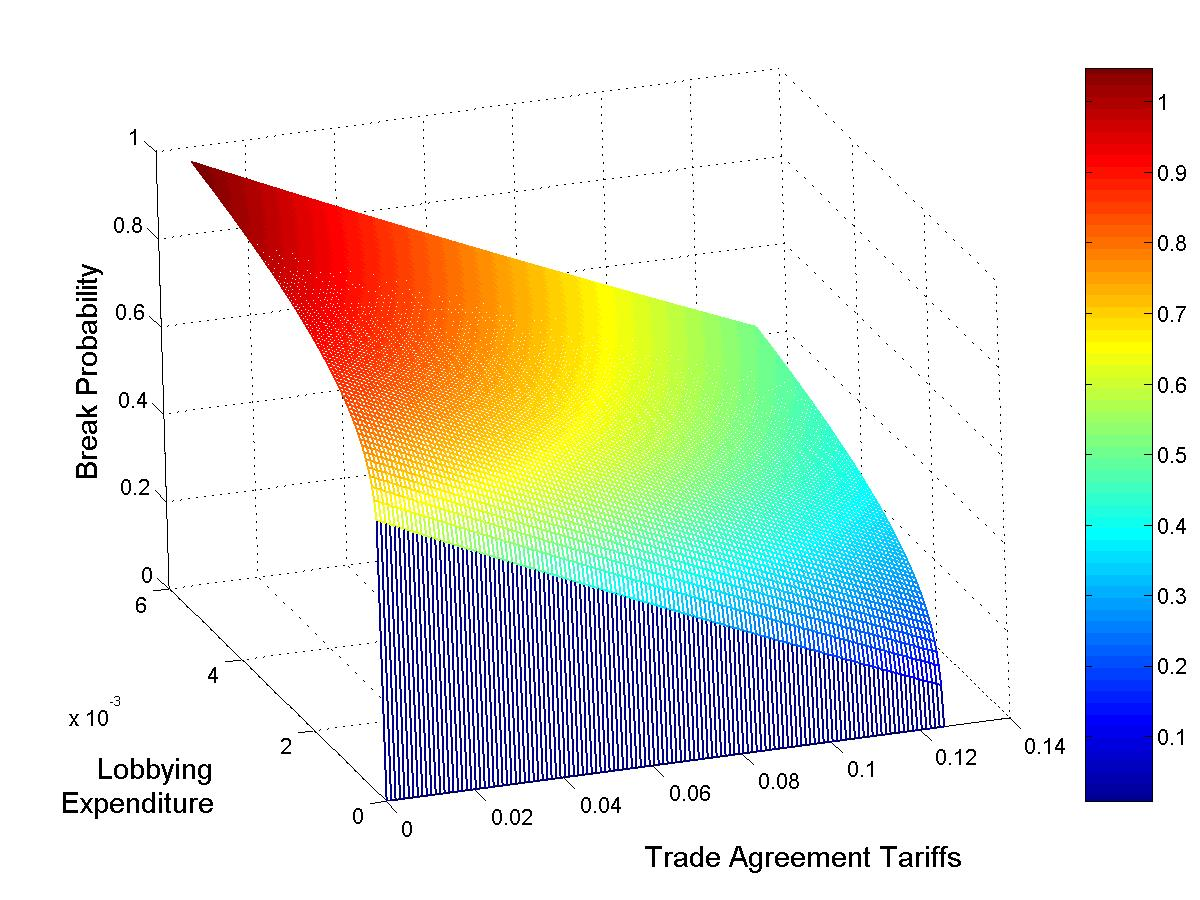
\includegraphics[height=3in, width=4in]{brprob2.jpg}
\end{center}
\caption{Probability Trade Agreement will be Broken\label{fig:br}}
\end{figure}

\begin{comment}
\begin{figure}
\begin{center}
\includegraphics[height=2.50in, width=3in]{contributions.jpg}
\end{center}
\caption{Lobbying Effort\label{fig:cont}}
\end{figure}
%graph is created in lobby_fix.m
\end{comment}

\begin{comment}
\begin{figure}
\centering
\begin{subfigure}{.5\textwidth}
  \centering
  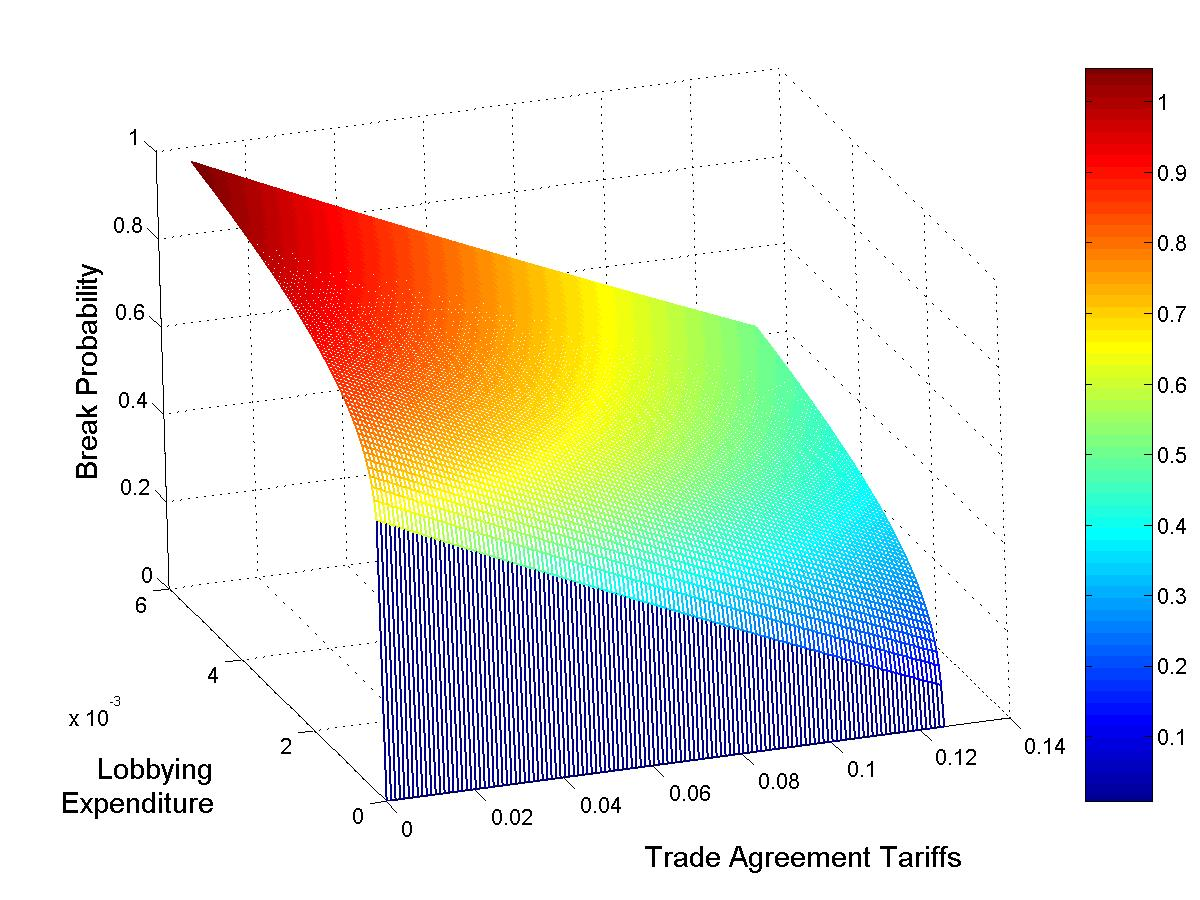
\includegraphics[width=.4\linewidth]{brprob2.jpg}
  \caption{Probability Trade Agreement will be Broken}
  \label{fig:br}
  %\label{fig:sub1}
\end{subfigure}%
\begin{subfigure}{.5\textwidth}
  \centering
  \includegraphics[width=.4\linewidth]{contributions.jpg}
  \caption{Lobbying Effort}
  \label{fig:cont}
  %\label{fig:sub2}
\end{subfigure}
%\caption{A figure with two subfigures}
%\label{fig:test}
\end{figure}
\end{comment}

Next we move to the legislature's decision on whether or not to break the trade agreement. Figure~\ref{fig:br} depicts the probability that the legislature will vote to break the trade agreement as a function of the tariff levels set in the trade agreement (with the restriction that $\tau^a = \tau^{*a}$) and the lobby's effort. It is strongly increasing in lobbying effort and decreasing in the level of tariffs set in the trade agreements.

Given the impact of lobbying on the legislature's break decision, the lobby's optimal contribution level is strongly decreasing in the trade agreement tariffs.%, as shown in Figure~\ref{fig:cont}.

\subsection{Trade Agreement}
Because the probability of legislative break never reaches zero for this parameterization, the executives' welfare function is concave everywhere. Assuming that each legislature has the opportunity to vote to break the agreement with probability $\frac{1}{2}$ and that the executives are social-welfare maximizers (i.e. $\ga_E = \ga_E^* = 1$), they will set trade agreements tariffs of $\tau^a = \tau^{*a} = 0.078$, with lobbying expenditures of $0.0007$ and a total break probability of $0.505$. The expected tariff is then $0.103$.

We can compare this against several different benchmarks. The most stark is the trade-war outcome itself, which can also be interpreted as the outcome that would prevail in the absence of executive involvement in trade policy \textit{and} the absence of any effort to make a trade agreement. The tariff in the executive-formed trade agreement is about 60$\%$ of the Nash tariff of $0.129$, and the expected level given the probability that the agreement will be broken is 80$\%$ of the Nash level. Lobbying expenditures in the agreement-maintenance phase are about 40$\%$ of the those in the Nash game, while expected expenditures in the executive-led trade-agreement scenario are 90$\%$ of what they would be if the legislatures set tariffs unilaterally.

Although the welfare-maximizing governments here are not able to set and maintain tariffs at zero as they would like, they are able to achieve significant reductions in tariff levels through the use of the trade agreement.

Another interesting benchmark is the scenario in which no executives are involved in trade policy, but in which the politically-susceptible legislatures can make use of a trade agreement. As in Bagwell and Staiger (2005), I find when maximizing their joint welfare in a legislature-led trade agreement ($W_{\mathit{ML}}(\tau, \tau^*) = W_{\mathit{ML}}^X(\tau) + W_{\mathit{ML}}^Y(\tau^*)$), the cooperative tariff levels will be set at
\[
  \tau^L = \frac{4\ga(e,\ve)-4}{25-4\ga(e,\ve)}, \ \tau^{*L} = \frac{4\ga(e^*,\ve)-4}{25-4\ga(e^*,\ve)}
\]
The legislatures are able to use the agreement to internalize the terms of trade externality, making political influence more expensive for the lobbies. Indeed, I find that lobbying expenditures rise to $0.0027$---60$\%$ higher than in the Nash case---while the agreement tariffs are set at $0.118$, only slightly lower than the Nash tariffs of $0.129$ and still higher than even the expected tariffs from the trade agreement scenario in which the executives choose the tariffs.

If one interprets the addition of a second policy-making actor as consistent with a move from autocracy to democracy, this result helps to explain the extensive empirical evidence that democracies trade more with each other than autocracies.\footnote{cfr. Laver and Shepsle (1991); Henisz and Mansfield (2006); Aidt and Gassebner (2010).}


\section{Discussion}
\label{sec:dis}

\subsection{Separation of Powers}
\label{sec:sep_powers}
Consider the model of Section~\ref{sec:main} for the case of $\ve_b=0$---that is, no uncertainty at the break stage (as will be discussed in Section~\ref{sec:uncertainty}, in the case of mean-zero uncertainty, strategic behavior at the trade-war stage is not altered by uncertainty). This allows the isolation of the results that derive from the assumption that power over trade policy is shared between the executive and legislative branches. Again, we focus on the home lobby.

Now $\ga(e_b)$ is deterministic, so the lobby knows the precise contribution it must make for any given trade agreement tariffs $\bta$ to induce the legislature to break the agreement (see Inequality~\ref{eq:lwcg}). Here, the lobby's contribution \textit{increases} in $\bta$ since the higher are the trade agreement tariffs, the larger is the political weight that is required to induce the legislature to find them unsatisfactorily low. As long as trade war profits net of the required contribution are greater than trade agreement profits, the lobby will induce a trade war; otherwise, it is not in the lobby's interest to make any contribution. Facing this behavior, the executives set the lowest trade agreement tariffs that make it prohibitively expensive for the lobby to have the agreement broken.

I return to the example of Section~\ref{sec:example} to illustrate the effects of changing the environment to one without political uncertainty. Recall that in the main example with $\ve$ distributed uniformly on $[-0.25,0.25]$, the expected Nash tariff is $0.129$ and the executive-led trade agreement tariff is $0.078$, with lobbying expenditures of $0.0007$ and a total break probability of $0.505$. The expected tariff is then $0.103$.

In this example, if the executives set the trade agreement facing no uncertainty, the tariff level is $0.106$, the lobby exerts zero effort, and the agreement remain in force with probability 1. If instead the executives were to set trade-agreement tariffs of $0.105$, the lobby would contribute $0.0025$ and the legislature would break the agreement with probability 1. This demonstrates both the agenda-setting power of the executives and the stark discontinuities induced when political uncertainty is not an issue.

Moreover, this case highlights the manipulation of the tariff level to discourage lobbying and therefore the disconnect that can arise between the tariffs that are chosen and the preferences of the governmental actors. In the example, the executive is a social welfare maximizer and so prefers zero tariffs, while the legislators with $\ga(e) = 1.25 + e^{.2}$ with $e_b = 0$ prefer $\tau^a = 0.05$. However, the trade agreement tariffs are set at $0.106$ precisely to ensure that $e_b =0$ so that we have a relatively free-trading legislature that upholds the agreement.


\subsection{Relation to Grossman and Helpman's `Protection for Sale'}
\label{sec:gh}
The legislative welfare function employed in this paper permits flexibility to take account of a wide range of political processes within a non-unitary legislature; alternatively, it can be a model of a unitary policy-maker when special interests face non-constant returns to lobbying activity. As noted in Section 2, the non-linear relationship between lobbying effort and tariffs follows Dixit, Grossman and Helpman (1997) and is a departure from the `Protection for Sale' welfare function, which assumes that a unitary government maximizes the sum of contributions and some fraction, $a$, of social welfare.

To see the relationship between the two forms, write the PFS welfare function (replacing $C$ with $e$) as
\[
  e + aW = e + a \left[ \mathit{CS}_X(\tau) + \mathit{PS}_X(\tau) + \mathit{CS}_Y(\tau^*) + \mathit{PS}_Y(\tau^*) + \mathit{TR}(\tau) \right]
\]
The relationship between $e$ and the weight the legislature places on profits is endogenous; because the PFS government welfare function has such an elegant and completely specified form, it is possible to solve for equilibrium behavior to retrieve this relationship directly.

It is easy to describe the equilibrium behavior and thus how lobbying effort will be related to the weight on profits in equilibrium in the PFS model when there is one lobby who makes a take-it-or-leave-it offer. Take the case of no uncertainty and assume that the legislature chooses $\tau=0$ in the absence of lobbying and that $\ga(0)=1$. For any $\tau$ that the lobby desires, it must pay according to the  indifference condition $e(\tau) = a \left[ W(0) - W(\tau) \right]$. That is, the lobby must pay for the $a$-weighted welfare loss caused by the tariff it requests.

In the model of this paper, this indifference condition, rearranged to solve for $\ga(e)$, is
		    \[
		      \ga(e) = \frac{\mathit{CS}_X(0) + \pi_X(0) + \mathit{CS}_Y(0) + \pi_Y(0) + \mathit{TR}(0) - \mathit{CS}_X(\tau) - \mathit{CS}_Y(\tau^*) - \pi_Y(\tau^*) - \mathit{TR}(\tau)}{\pi_X(\tau)}
		    \] 
In order to match the form of the PFS framework, we must therefore have
		    \begin{equation}
		      \ga(e) = 1 + \frac{e}{a\pi_X(\tau)}
		      \label{eq:gh}
		    \end{equation}

Choosing the political weighting function identified in Equation~\ref{eq:gh} aligns the political objective function used in the current model with the PFS framework. Although using the $\ga$-weighted government welfare function is a reduced-form approach in the sense that legislative dynamics are not fully modeled, a drawback of the PFS welfare function is that it embodies the restriction that returns to lobbying effort must be constant.

As noted in Dixit, Grossman and Helpman (1997), the linear form also implies transferable utility between the lobby and unitary government; this leads to equilibrium indeterminancies and an inability to speak to distributional questions, prompting them to generalize the PFS form. From their results, we have that the same equilibrium analysis holds in the more general environment.

For the trade policy literature, generalizing the linear form in a sense would obviate many of the questions that have been raised by empirical investigations of the PFS model about the relationship of the magnitude of welfare losses relative to the weight placed on social welfare by governments as the $a$ parameter for the constant relative marginal utility provided by social welfare would no longer be present in the model.

The linear PFS form provides for an almost unmatched simplicity and elegance that is able to capture the key cross-industry predictions on import tariffs. A perhaps unintended byproduct in the subsequent literature seems to have arisen in the form of a focus on matching fine details of governments' welfare-mindedness using a model that has a very simple unitary government and is thus better suited for other purposes.

It is clear that trade policy is often shaped in a complicated process involving multiple actors (see, for instance, Destler (2005) for the U.S.). The model presented herein is a first attempt to more richly model the policy-making process and thus shed light on open questions surrounding how government preferences and the details of political institutions impact trade policy outcomes.


\subsection{The Role of Political Uncertainty}
\label{sec:uncertainty}
In this model, if there were no political uncertainty, there would be no lobbying in equilibrium. Thus, if nothing else, adding the realism of political uncertainty allows for positive lobbying on the equilibrium path. If we examine more closely the assumption that there is significant uncertainty surrounding the legislative lobbying process, additional insights come to light. It is most clear in the case of mean-zero uncertainty, so I will assume this throughout this section unless otherwise noted.

In the event of a trade war, the lobbies' behavior, and therefore the expected trade-war tariffs, are not altered by mean-zero uncertainty (see Equation~\ref{eq:lobtw}).

At the earlier stage of lobbying, uncertainty alters optimizing behavior by both the lobby and the executives. In contrast to the previous section with no uncertainty, consider adding a very small amount of uncertainty to the previous example: take $\ve$ distributed uniformly on $[-0.01,0.01]$. Here, the executives find it optimal to set the tariffs to completely disengage the lobby and ensure the agreement remains in force. However, the tariff level will be different because instead of making the decision to lobby according to the certainty condition
\[\pi(\tau^n) - e_n - \pi(\tau^a) > e_b,
\]
the lobby makes this decision according to Condition~\ref{ine:lobint}, which can be re-written as
\[
\pi(\tau^n) - e_n - \pi(\tau^a) > \left[\frac{\partial b(0,\bta,\btn(e_n,e_n^*))}{\partial e_b}\right]^{-1}.
\]

Although the relationship between the tariff under certainty and a small amount of uncertainty will depend on the structure of the economy and the legislative process, in this case, the tariff can be reduced slightly to $0.105$. As we have seen above, with significant uncertainty, the tariff in this example is reduced to $0.078$. Interestingly, the optimal tariff does not decrease monotonically between these two values as uncertainty increases.

\begin{figure}
\begin{center}
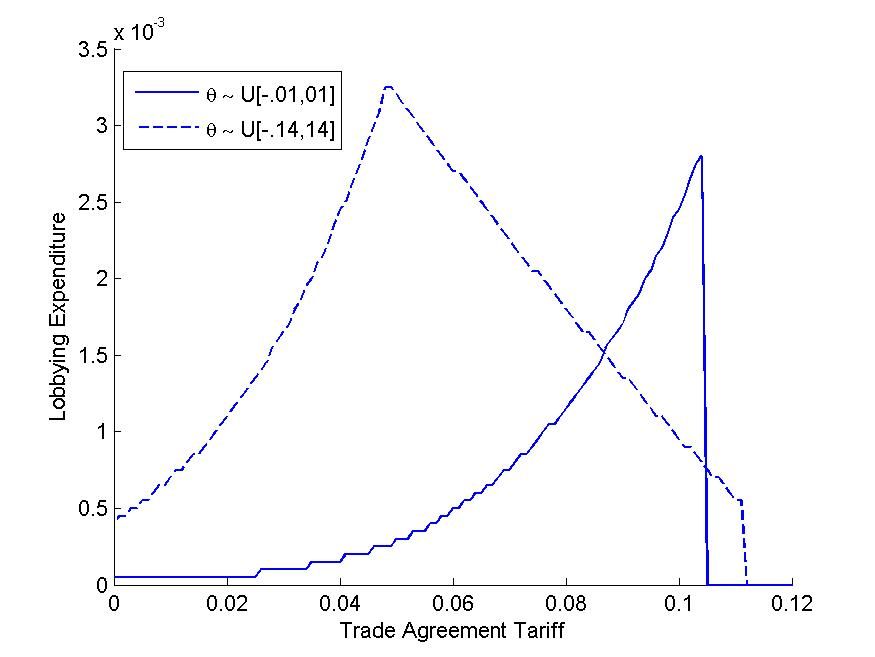
\includegraphics[height=3in, width=4in]{lobby_br.jpg}
\end{center}
\caption{Lobby's Optimal Expenditure Function (Low and Intermediate Uncertainty)\label{fig:lobby_br}}
\end{figure}

It is particularly instructive to examine the lobby's reaction function at this very low level of uncertainty as well as the intermediate level when $\ve$ is distributed uniformly on $[-0.14,0.14]$ because it is at the latter that the executives set the highest tariff level of $0.107$. For the former, when facing very little uncertainty, the range of tariff levels to which the lobby responds with an intermediate contribution that leaves open the possibility of a break is very small: only those between 0.103 and 0.104. The lobby disengages completely at $\bta=0.105$ (see Figure~\ref{fig:lobby_br}).

In contrast, when uncertainty is increased to the interval $[-0.14,0.14]$, the lobby begins to leave open the possibility of a break at $\bta = 0.048$. It disengages at $0.107$ and this is the tariff level that the executives find optimal. Interestingly, at intermediate uncertainly levels, both portions of the best response curve are steeper and the lobby disengages at slightly lower tariff levels---as low as $0.099$ when $\ve \sim U[-0.06,0.06]$.

The preceding discussion illustrates Part (a) of Result~\ref{res:execsoln}: here the executives maximize their welfare by raising tariffs to the point where the import-competing industry ceases to lobby and thus the agreement remains in force for sure. Note, however, that although lobbying expenditures are zero, the potential for lobbying behavior is essential in shaping the trade agreement.

%\begin{figure}
%\begin{center}
%\includegraphics[height=3.8in, width=7in]{exec_welfare.jpg}
%\end{center}
%\caption{Differences in Executive Welfare when Uncertainty Increases\label{fig:exec_wel}}
%\end{figure}

When uncertainty rises above this threshold of $\ve \sim U[-0.14,0.14]$, the executives' choices are made according to Part (b) of Result~\ref{res:execsoln}: that is, they trade off reductions in welfare under the agreement with reductions in the probability that the agreement will be abrogated by the legislature. %In terms of the lobby's best response function, the executives now choose the optimal point on the downward-sloping portion of the curve instead of the point where it reaches zero. In terms of the welfare function for the executives, shown in Figure~\ref{fig:exec_wel}, they are now choosing the point that maximizes the concave portion of the curve instead of the ``spike'' that is created when the lobbies disengage and the chance that the agreement will be abrogated is removed altogether.\footnote{Note that the initial, flat portion of the curve is where the tariff is low enough that the lobby buys a trade war with certainty; we then enter the concave portion where the main results of Section~\ref{sec:main} are applicable; finally, we see the upward spike where the probability of a trade war is reduced to zero and the executives' welfare declines after that because there is no further reduction in break probability as the tariff increases.}

As uncertainty increases further, the general pattern is that tariffs, and therefore lobbying effort, are reduced, while the break probability increases. However, this pattern is not smooth or absolute, in contrast to the welfare level achieved by the executives, which increases monotonically in the amount of uncertainty present. %It is not clear how general a result this is, but it is particularly interesting in contrast to the non-monotone pattern over the lower-range of uncertainty where executive welfare is minimized at the edges of the range that lead to disengagement of the lobby and maximized in the middle of that range.

Several salient points emerge from this example. First, different amounts of uncertainty lead to very different outcomes---both in terms of the tariffs that are set in the trade agreement and the probability of disruption. Second, these outcomes vary in nuanced ways with the underlying behavior of the lobbies and the executives. The provided tariff levels are strongly influenced by lobbying incentives, but not in the straightforward ways predicted by unitary models.

\begin{comment}
\section{Extensions}
\label{sec:ext}

This analysis has been undertaken with the assumption that the import-competing industry is distributed evenly across legislative districts. By varying the way in which those profits enter the welfare function of the median legislator (before lobbying takes place), I can provide results about how district composition affects trade policy.

There are also several directions to explore in comparing different government structures. I start by describing the value of a trade agreement in an institutional setting of divided government.
\begin{result}
  Lobbying effort is reduced by the presence of executive branches who form a trade agreement (where the counterfactual is legislatures setting unilateral trade policy).
\end{result}
\textcolor{blue}{Don't yet know what assumptions I need to make this work} \\

Comparing this model to the unitary-government model is a delicate task. The most straightforward approach from the current structure is to disregard the executives and allow the legislative branches to form a trade agreement cooperatively after lobbying takes place. Note that we can retain the stochastic nature of the tariff-setting, but there is no vehicle for the agreement to be broken. In this case, the trade agreement tariff in home, $\tau_U^a$ will maximize
\[
  W_X(\tau,\ga_E) + W_X^*(\tau) = \frac{9}{98} - \frac{5}{49}\tau - \frac{34}{49}\tau^2 +\frac{1}{98}\ga(e,\ve)\left[ 8 + 16\tau + 8\tau^2 \right] + \frac{25}{98} - \frac{3}{49}\tau + \frac{9}{49}(\tau)^2 
\]
and will thus be set at
\[
  \tau_U^a = \frac{4\ga(e,\ve)-4}{25-4\ga(e,\ve)}.
\]
$\tau_U^a < \tau^n$ for all $\ga(e,\ve) < 7/4$, while $\ga(e,\ve)=7/4$ results in the prohibitive tariff of $1/6$. This is the standard result that a trade agreement internalized the terms of trade externality and results in a lower tariff than unilateral policy making. 

\textcolor{blue}{will an executive inserted into this situation set higher or lower tariffs, what will happen to $e$?}

What if we add executive branches with essentially the same preferences as the legislature? That is, set $\ga_E = \expect[\ga(e,\ve)]$. \textcolor{blue}{It's hard to say how $e$ should be chosen here...still need to figure that out. But if we can get around the weird time inconsistency problem...} What agreement tariffs will the executives choose? It's easy to see that they will not choose $\tau^a < \tau_U^a$, as $\tau_U^a$ is their ideal point if there were no possibility of the agreement being broken, and lower tariffs only incentivize more lobbying and a higher probability that the agreement will be broken.

Thus, if an interior solution exists \textcolor{blue}{[should have conditions to insert here]}, the executive will exploit the same trade-off explored earlier, raising $\tau^a$ a bit to reduce the probability that the agreement will be abrogated. So interestingly, we can see that executives with the same political preferences as the legislature will choose higher trade agreement tariffs than the legislature would by itself due to the possibility that the agreement can be broken and the impact of the tariff choice on lobbying. We will also therefore have a reduced level of contributions, and if a trade war were possible, lower trade war tariffs because of it.

Along these lines, allowing for asymmetries in the preferences and political processes between the countries will provide important insights as well.

I also plan to use the richness of this model to parse out how much of the changes in tariffs comes from the fact that the executives place lower weight on producer profits and how much comes from the fact that they make an agreement---that is, compare the effects of structure versus preferences.



\subsection{Asymmetric Trade Agreements}
\label{sec:asym}
The assumption that the legislatures do not have the opportunity to break a trade agreement simultaneously serves to simplify the analysis of the interaction between the lobbies and the consequences of relaxing it will be discussed in the following section. Maintaining it for now, however, facilitates examination of the assumption that trade agreements must be symmetric. This may be quite realistic in some settings where additional political constraints would make ``unfair'' arrangements unpalatable. However, it is important to point out that, for some parameter choices, the joint welfare of the executives is in fact maximized by an asymmetric agreement.

The parameterization from the example in Section~\ref{sec:example} is one such instance. The optimal unrestricted trade agreement is to set tariffs in one country (say home) at $0.062$ and those in the other (foreign) at 0. In this case, the equilibrium break probability in home, if the home legislature is afforded the opportunity, is zero, while the foreign legislature will break the agreement with probability 1 if given the chance. With the assumption from the example that each legislature gets the opportunity to repudiate the agreement half the time, this results in the trade agreement being broken with probability $0.50$, just less than the $0.505$ of the optimal symmetric agreement with both tariffs set at $0.078$. Because both the trade agreement tariffs and the expected chance that the agreement will remain in force are lower, expected welfare for the executives is higher.

What is behind the rather surprising result that a lower break probability can be achieved when both tariffs are strictly lower than in the symmetric agreement? Here, the executives relinquish any chance of passage of the trade agreement in the foreign country (in essence hoping that its legislature will not have a chance to act). Once they decide to pursue this course, it is optimal to reduce $\tau^{*a}$ to zero. This drastically reduces the home legislature's incentive to break the trade agreement. Because of the large direct impact of $\tau^{*a}$ in reducing the break probability, the home tariff is not required to make such a large contribution and can be lowered, which in turn reduces the lobby's incentive to exert effort (see Result~\ref{res:lobby}). This effect is strong enough that the executives can set a tariff level lower than that of the symmetric agreement that is sufficient to disengage the home lobby (see Inequality~\ref{ine:lobint}). 

It is useful to keep in mind that this result occurs in a completely symmetric environment. Recall that, in general, the executives maximize joint welfare in Equation~\ref{eq:jv2}. If the chance that the legislatures will have the opportunity to break the agreement ($o$ and $o^*$) are not equal, or if another significant aspect of the economic or political situation is asymmetric, the importance of this result grows in a potentially substantial way. In particular, if only one country faces a legislative constraint, an asymmetric agreement seems highly likely as in the large body of literature investigating the Schelling conjecture.


\subsection{Break Opportunities in Both Countries}
\label{sec:two}
Although it changes their expected payoffs, extending the model to allow both legislatures the opportunity to break the trade agreement simultaneously does not impact the legislatures' incentives as each decision to break or not break the agreement is independent of the other.

However, the lobbies' incentives are altered because the total probability of a break with which they weight profits changes. Now, in addition to their own effort positively influencing their own legislature to break the agreement, the probability of a break in the trade agreement also increases in the effort of the other country's lobby. As might be expected, the lobbying effort in each country turns out to be a negative function of that in the trading partner; that is, to some extent, the lobbies have an incentive to free ride.

Without making stronger assumptions, it is not possible to say how much the effort of each lobby will be reduced therefore whether total lobbying effort rises or falls. What is clear is that the optimization of the executives becomes significantly more complex as they are now faced with the problem of how to best exploit the free-riding dynamics that occur between the lobbies. 
\end{comment}

\section{Conclusion}
\label{sec:concl}
I have shown that the legislature both breaks trade agreements with a higher probability and sets higher trade war tariffs when lobbying activity increases, while the probability with which it breaks agreements (or fails to ratify them) decreases in the domestic trade agreement tariff. Because the lobby decreases its effort in response to higher trade agreement tariffs, the executives face a trade-off between the welfare derived while a trade agreement is in force and the probability with which the agreement actually enters into force.

I have also shown that in a policy-making structure in which power is shared, a less politically-motivated executive can utilize an international trade agreement to reduce the political pressure on the ratifying body and therefore increase the probability that the agreement will remain in force. Thus, in a model with a richer description of government structure, a political-commitment role for trade agreements can arise.

The executives' incentive to raise tariffs in order to reduce lobbying effort helps to explain the empirical finding in the Protection for Sale literature that levels of protection and associated deadweight losses are too high relative to lobbying expenditure given the high estimates for governments' weighting of social welfare. I have shown that this serves to mediate the relationship between preferences for contributions relative to social welfare and the tariffs that are provided. The intuition is clear: the observed lobbying expenditure levels may in fact be low \textit{because} tariffs have been raised sufficiently high to prevent political pressure and the increased risk of a costly trade disruption it engenders.

That lobbying and tariff levels are related in systematic ways to the amount of political uncertainty present suggests interesting avenues for future empirical work. Several directions for future theoretical work also seem potentially fruitful, including removing the assumption of perfect enforceability and supporting cooperation through repeated interaction and generalizing the model to the case of multiple lobbies.

			




\section{Appendix}
\label{sec:appendix}
\noindent \textbf{\hypertarget{Pr_bincC}{Proof of Result~\ref{res:bincC}}}:\\
Substituting from Equation~\ref{eq:ml}, Equation~\ref{eq:b} can be re-written as
\begin{multline}  
  b(e_b,\bta,\btn) = \Pr [ \mathit{CS}_X(\tau^n) + \ga(e_b,\ve_b) \cdot \mathit{PS}_X(\tau^n) + \mathit{CS}_Y(\tau^{*n}) + \mathit{PS}_Y(\tau^{*n}) + \mathit{TR}(\tau^n) >  \\ \mathit{CS}_X(\tau^a) + \ga(e_b,\ve_b) \cdot \mathit{PS}_X(\tau^a) + \mathit{CS}_Y(\tau^{*a}) + \mathit{PS}_Y(\tau^{*a}) + \mathit{TR}(\tau^a) ]
\end{multline}
Rearranging, we have $b(e_b,\bta,\btn) = $
\begin{multline}  
  \textstyle \Pr \Big[ \frac{\mathit{CS}_X(\tau^n) + \mathit{PS}_X(\tau^n) + \mathit{CS}_Y(\tau^{*n}) + \mathit{PS}_Y(\tau^{*n}) + \mathit{TR}(\tau^n)  -\mathit{CS}_X(\tau^a) - \mathit{PS}_X(\tau^a) - \mathit{CS}_Y(\tau^{*a}) - \mathit{PS}_Y(\tau^{*a}) - \mathit{TR}(\tau^a)}{\mathit{PS}_X(\tau^a) - \mathit{PS}_X(\tau^n)} + 1 \\ \textstyle < \ga(e_b,\ve_b) \Big]
  \label{eq:b_ex}
\end{multline}
%\noindent The left side of the inequality in Expression~\ref{eq:b_ex} does not depend on $e_b$. By Assumption~\ref{as:ga_c}, the right side of the inequality is increasing and concave in $e_b$. Thus $b(e_b,\bta,\btn)$ is increasing and concave in $e_b$.    $\hfill\blacksquare$
\noindent The left side of the inequality in Expression~\ref{eq:b_ex} does not depend on $e_b$. Call it $Z$. Thus we have $b(e_b,\bta,\btn) = \Pr [Z < \ga(e_b,\ve_b) ] = 1 - F_{\ga}(\ga=Z)$ where $F_{\ga}(\ga=Z) = F_{\ta}(\ta=h^{-1}(\ga,e))$ by the Change of Variables Theorem and Assumption~\ref{as:ga_ta} with $\ga = h(e,\ta)$ giving the change of variable.

Then $\frac{\partial b}{\partial e} = -\frac{\partial F_{\ta}(\ta=h^{-1}(\ga,e))}{\partial \ta}\frac{\partial h^{-1}(\ga,e)}{\partial e} = -f_\ta(\ta) \frac{\partial h^{-1}(\ga,e)}{\partial e}$ and $\frac{\partial^2 b}{\partial e^2} = -f_\ta(\ta) \frac{\partial^2 h^{-1}(\ga,e)}{\partial e^2}$. Because $\ga = h(e,\ta)$ is increasing and concave in $e \ \forall \ta$ by Assumption~\ref{as:ga_c}, its inverse is decreasing and convex $\left(\frac{\partial h^{-1}(\ga,e)}{\partial e}\leq 0; \ \frac{\partial^2 h^{-1}(\ga,e)}{\partial e^2} \geq 0 \right)$ The pdf of $\ta$ is non-negative, so $\frac{\partial b}{\partial e} \geq 0$ and $\frac{\partial^2 b}{\partial e^2} \leq 0$. $\hfill\blacksquare$

\vskip.4in
\noindent \textbf{\hypertarget{Pr_leg_astar}{Proof of Lemma~\ref{lem:leg_astar}}}:\\
It must be shown that the left hand side of the inequality in Expression~\ref{eq:b_ex} is decreasing in $\tau^{*a}$. The derivative of this quantity with respect to $\tau^{*a}$ is 
\begin{equation}
  \frac{-\left(\mathit{PS}_X(\tau^a) - \mathit{PS}_X(\tau^n)\right)\left(\frac{\partial \mathit{CS}_Y(\tau^{*a})}{\partial \tau^{*a}} + \frac{\partial \mathit{PS}_Y(\tau^{*a})}{\partial \tau^{*a}}\right)}{\left(\mathit{PS}_X(\tau^a) - \mathit{PS}_X(\tau^n)\right)^2} = \frac{\frac{\partial \mathit{CS}_Y(\tau^{*a})}{\partial \tau^{*a}} + \frac{\partial \mathit{PS}_Y(\tau^{*a})}{\partial \tau^{*a}}}{\mathit{PS}_X(\tau^n) - \mathit{PS}_X(\tau^a)}.
  \label{appex:astar}
\end{equation}

\noindent The price of good $Y$ is decreasing in $\tau^{*a}$, so consumer surplus is increasing and producer surplus is decreasing in $\tau^{*a}$. Because $Y$ is being exported, the decrease in producer surplus is larger than the increase in consumer surplus, making the numerator negative. Since producer surplus in the denominator is increasing in $\tau$, the expression in Equation~\ref{appex:astar} is negative for all $\tau^{*a}$.  $\hfill\blacksquare$


\vskip.4in
\noindent \textbf{\hypertarget{Pr_leg_a}{Proof of Lemma~\ref{res:leg_a}}}:\\
Using the logic of the proof of Lemma~\ref{lem:leg_astar}, the effect on the break probability is determined by the sign of the derivative of the left hand side of the inequality in Expression~\ref{eq:b_ex} with respect to $\tau^a$; to show that the break probability is decreasing in $\tau^a$, I must demonstrate that this derivative is positive. Labeling the numerator of that expression $\left[ W(\btn)-W(\bta)\right]$ (for the change in social welfare), this derivative can be written
\begin{equation}
  \frac{\left(\mathit{PS}_X(\tau^n) - \mathit{PS}_X(\tau^a)\right)\left(\frac{\partial \mathit{CS}_X(\tau^{a})}{\partial \tau^{a}} + \frac{\partial \mathit{PS}_X(\tau^a)}{\partial \tau^{a}} + \frac{\partial \mathit{TR}(\tau^{a})}{\partial \tau^{a}}\right) - \left[ W(\btn)-W(\bta)\right] \frac{\partial \mathit{PS}_X(\tau^a)}{\partial \tau^a}}{\left(\mathit{PS}_X(\tau^a) - \mathit{PS}_X(\tau^n)\right)^2}.
  \label{appex:a}
\end{equation}

\noindent $\left(\mathit{PS}_X(\tau^n) - \mathit{PS}_X(\tau^a)\right)$ is always positive by Assumption~\ref{as:ga_l_e}. Because the optimal unilateral tariff for large welfare-maximizing governments is positive (call it $\tau^O$), $\left(\frac{\partial \mathit{CS}_X(\tau^{a})}{\partial \tau^{a}} + \frac{\partial \mathit{PS}_X(\tau^a)}{\partial \tau^{a}} + \frac{\partial \mathit{TR}(\tau^{a})}{\partial \tau^{a}}\right)$ is increasing up to $\tau^O$ and decreasing above it. Thus the first summand is increasing up until $\tau^O$ and decreasing thereafter.

Because total social welfare is maximized at $\tau^a = \tau^{*a} = 0$, $W(\btn)-W(\bta)$ is always negative, whereas producer surplus is increasing in $\tau^a$, so the second summand is positive everywhere. With a positive denominator, we thus have that the derivative is positive on $[0,\tau^O]$.

It is also positive over the remaining $(\tau^O,\tau^n)$. To see this, add $\left(\tilde{\Gamma} - 1 \right) \frac{\partial \mathit{PS}_X(\tau^a)}{\partial \tau^a} \left(\mathit{PS}_X(\tau^n) - \mathit{PS}_X(\tau^a)\right)$ to the first summand and subtract it from the second. For any particular value of $\tilde{\tau}^a$, one can choose the $\tilde{\Gamma}$ weight that would make $\tilde{\tau}^a$ the preferred unilateral tariff; this makes the derivative in the first summand zero. Having subtracted the same quantity from the second summand modifies the welfare difference in the second summand to be maximized at $\tilde{\tau}^a$ so that this term is always negative, thus ensuring the result.  $\hfill\blacksquare$


\vskip.4in
\noindent \textbf{\hypertarget{Pr_bcomb}{Proof of Lemma~\ref{res:bcomb}}}:\\
Again, I want to show how the inequality in Expression~\ref{eq:b_ex} changes, now with respect to both $\tau^a$ and $\tau^{*a}$, so I add the derivatives in Expressions~\ref{appex:astar} and \ref{appex:a} to get
\[
  \frac{\left(\mathit{PS}_X(\tau^n) - \mathit{PS}_X(\tau^a)\right)\left(\frac{\partial \mathit{W}_X(\bta)}{\partial \tau^{a}} + \frac{\partial \mathit{W}_X(\bta)}{\partial \tau^{*a}}\right) - \left[ W(\btn)-W(\bta)\right] \frac{\partial \mathit{PS}_X(\tau^a)}{\partial \tau^a}}{\left(\mathit{PS}_X(\tau^n) - \mathit{PS}_X(\tau^a)\right)^2}.
\]
where $\frac{\partial \mathit{W}_X(\bta)}{\partial \tau^{a}} + \frac{\partial \mathit{W}_X(\bta)}{\partial \tau^{*a}} = \frac{\partial \mathit{CS}_X(\tau^{a})}{\partial \tau^{a}} + \frac{\partial \mathit{PS}_X(\tau^a)}{\partial \tau^{a}} + \frac{\partial \mathit{TR}(\tau^{a})}{\partial \tau^{a}} + \frac{\partial \mathit{CS}_Y(\tau^{*a})}{\partial \tau^{*a}} + \frac{\partial \mathit{PS}_Y(\tau^{*a})}{\partial \tau^{*a}}$ is the total derivative of social welfare. Since social welfare is maximized at $\bta = (0,0)$,\footnote{Note, this is identical to the result that joint social welfare is maximized at zero tariffs because of symmetry.}  this is negative $\forall \bm{\tau} \in (\bm{0},\btn]$; note that it is 0 at $\bm{0}$ and vanishingly small for very small tariffs.

Thus the first summand in the numerator is zero at $\bta = \bm{0}$ and increasingly negative as $\bta$ increases. The second summand is positive everywhere because social welfare, $W$, is lowest at $\btn$ and producer surplus is increasing everywhere. Thus the numerator is positive at $\bm{0}$ and at least for very small $\bta$

It is also positive for all other values of $\bta$ strictly below $\btn$. Just as in the proof of Lemma~\ref{res:leg_a}, one can add
$\left(\tilde{\Gamma} - 1 \right) \frac{\partial \mathit{PS}_X(\tau^a)}{\partial \tau^a} \left(\mathit{PS}_X(\tau^n) - \mathit{PS}_X(\tau^a)\right)$ to the first summand and subtract it from the second. For any particular value of $\tilde{\bta}$, one can choose the $\tilde{\Gamma}$ weight that would make $\tilde{\bta}$ the politically optimal tariff; this makes the derivative in the first summand zero. Having subtracted the same quantity from the second summand modifies the welfare difference in the second summand to be maximized at $\tilde{\bta}$ so that this term is always negative, thus ensuring the result.

Because the denominator is positive, the entire expression is positive for all $\bta < \btn$.   $\hfill\blacksquare$


\vskip.4in
\noindent \textbf{\hypertarget{Pr_lobby}{Proof of Result~\ref{res:lobby}}}:\\
Proof is via the Implicit Function Theorem using the lobby's first order condition, Equation~\ref{eq:lobbyfoc}, referred to here as $FOC_L$.
  \[
		\frac{\partial e_b}{\partial \tau^a} + \frac{\partial e_b}{\partial \tau^{*a}} = - \left[ \frac{\frac{\partial FOC_L}{\partial \tau^a}}{\frac{\partial FOC_L}{\partial e_b}} + \frac{\frac{\partial FOC_L}{\partial \tau^{*a}}}{\frac{\partial FOC_L}{\partial e_b}} \right] = \frac{ \frac{\partial b}{\partial e_b} \frac{\partial \pi(\bta)}{\partial \tau^a} + \frac{\partial b}{\partial e_b} \frac{\partial \pi(\bta)}{\partial \tau^{*a}} - \left\{\frac{\partial^2 b}{\partial e_b \partial \tau^a} + \frac{\partial^2 b}{\partial e_b \partial \tau^{*a}}   \right\}\left[ \pi(\tau^n) - e_n - \pi(\tau^a) \right]}{\frac{\partial^2 b}{\partial e_b{}^2} \left[ \pi(\tau^n) - e_n - \pi(\tau^a) \right]}
	\]
Beginning with the denominator: because $\pi(\tau)$ is increasing everywhere, $\left[\pi(\tau^n) - e_n - \pi(\tau^a) \right]$ is positive for all but very large values of $\tau^a$, that is for all $\tau^a$ such that $\pi(\tau^n) - e_n > \pi(\tau^a)$. When $\tau^a$ rises above this level, it is no longer in the lobby's interest to ask to have the agreement broken so $e_b=0$ and $\frac{\partial e_b}{\partial \tau^a} = 0$. $\frac{\partial^2 b}{\partial e_b{}^2}$ negative by Result~\ref{res:bincC}, so the denominator is negative for all values of $\tau^a$ at which $e_b$ is not constant.

$\frac{\partial b}{\partial e_b}$ is positive, $\frac{\partial \pi(\bta)}{\partial \tau^a}$ is positive by construction, and $\frac{\partial \pi(\bta)}{\partial \tau^{*a}}$ is zero: separability between the sectors implies that profits in the import-competing sector do not depend on $\tau^{*a}$. 

We can rewrite $\frac{\partial b(e,\bta)}{\partial  \tau^a} + \frac{\partial b(e,\bta)}{\partial  \tau^{*a}} = -\frac{\partial F_\ga (Z(\bta))}{\partial \tau^a} -\frac{\partial F_\ga (Z(\bta))}{\partial \tau^{*a}} = -\frac{\partial F_\ga (Z(\bta))}{\partial Z(\bta)}\left[\frac{\partial Z(\bta)}{\partial \tau^a} + \frac{\partial Z(\bta)}{\partial \tau^{*a}} \right] = - f_\ga \left[\frac{\partial Z(\bta)}{\partial \tau^a} + \frac{\partial Z(\bta)}{\partial \tau^{*a}} \right]$, where $F_\ga (Z(\bta))$ is the CDF of $\ga$ and $f_\ga (Z(\bta))$ is the pdf of $\ga$ and $Z(\bta)$ represents the left hand side of the inequality in Expression~\ref{eq:b_ex}.
	
Then $\frac{\partial^2 b}{\partial e_b \partial \tau^a} + \frac{\partial^2 b}{\partial e_b \partial \tau^{*a}} = 	- \frac{\partial}{\partial e} \left( \frac{\partial F_\ga (Z(\bta))}{\partial \tau^a} + \frac{\partial F_\ga (Z(\bta))}{\partial \tau^{*a}} \right) = 
	   - f_\ga \left[\frac{\partial^2 Z(\bta)}{\partial \tau^a \partial e} + \frac{\partial^2 Z(\bta)}{\partial \tau^{*a} \partial e} \right] - \left[\frac{\partial Z(\bta)}{\partial \tau^a} + \frac{\partial Z(\bta)}{\partial \tau^{*a}} \right] \frac{\partial f_\ga}{\partial e} = - \left[\frac{\partial Z(\bta)}{\partial \tau^a} + \frac{\partial Z(\bta)}{\partial \tau^{*a}} \right] \frac{\partial f_\ga}{\partial e} 
$
where the above equality holds because $Z(\bta)$ does not depend on $e$. Lemma~\ref{res:bcomb} shows that $\frac{\partial Z(\bta)}{\partial \tau^a} + \frac{\partial Z(\bta)}{\partial \tau^{*a}} \geq 0$, so $\frac{\partial f_\ga}{\partial e} \geq 0$ ensures that $\left\{\frac{\partial^2 b}{\partial e_b \partial \tau^a} + \frac{\partial^2 b}{\partial e_b \partial \tau^{*a}} \right\} \geq 0$. Thus $\frac{\partial e_b}{\partial \tau^a} + \frac{\partial e_b}{\partial \tau^{*a}} \leq 0$.  $\hfill\blacksquare$




\vskip.4in	  	
\noindent \textbf{\hypertarget{Pr_bcomB}{Proof of Result~\ref{res:bcomB}}}: \\
$	\frac{\partial B(\bta)}{\partial \tau^a} + \frac{\partial B(\bta)}{\partial  \tau^{*a}} = \frac{\partial b}{\partial  e_b}\frac{\partial e_b}{\partial \tau^a} + \frac{\partial b}{\partial  e_b}\frac{\partial  e_b}{\partial  \tau^{*a}} + \frac{\partial b}{\partial \tau^a} + \frac{\partial b}{\partial  \tau^{*a}} = \frac{\partial b}{\partial  e_b} \left\{ \frac{\partial e_b}{\partial \tau^a} + \frac{\partial  e_b}{\partial  \tau^{*a}} \right\} + \frac{\partial b}{\partial \tau^a} + \frac{\partial b}{\partial  \tau^{*a}}.$ $\frac{\partial b}{\partial  e_b}$ is positive by Result~\ref{res:bincC}. $\left\{ \frac{\partial e_b}{\partial \tau^a} + \frac{\partial  e_b}{\partial  \tau^{*a}} \right\}$ is negative by Result~\ref{res:lobby}. Taken together, the final two summands are negative by Lemma~\ref{res:bcomb}. Thus the entire expression is negative.   $\hfill\blacksquare$


\vskip.4in
\noindent \textbf{\hypertarget{int_soln}{Conditions for Interior Solution to Executives' Problem}} \\
The first order condition for maximizing joint surplus with respect to $\tau^a$ and $\tau^{*a}$ when the two are constrained to be equal is
\begin{multline*}
  \textstyle \left\{ 1 - o \cdot B(\bta) - o^* \cdot B^*(\bta) \right\} \left\{\frac{\partial \bm{W_E}(\bta)}{\partial \tau^a} + \frac{\partial \bm{W_E}(\bta)}{\partial \tau^{*a}} \right\} \\
     \textstyle + \left\{ o \cdot \left[\frac{\partial B(\bta) }{\partial \tau^a} + \frac{\partial B(\bta) }{\partial \tau^{*a}} \right] + o^* \cdot \left[\frac{\partial B^*(\bta)}{\partial \tau^a} + \frac{\partial B^*(\bta)}{\partial \tau^{*a}} \right] \right\} \left[ \bm{W_E}(\btn)- \bm{W_E}(\bta) \right] = 0
\end{multline*}
Because there is no benefit to setting $\bta$ below the executives' preferred level, which I will denote $\bm{\tau^E}$, I will take the choice space to be $[\bte,\btn]$. Note that for $\ga_E = 1$, $\bte=0$.

To demonstrate that the executives do not choose $\bta=\bte$, I must show that the left side of the above equation is positive at $\bta=\bte$. Assumption~\ref{as:ga_l_e} and Result~\ref{res:bcomB} combined with symmetry ensure that the first term of the second summand is negative. That executive welfare is maximized at $\bte$ ensures that the term multiplying it is also negative as well as that $\frac{\partial \bm{W_E}(\bte)}{\partial \tau^a} + \frac{\partial \bm{W_E}(\bte)}{\partial \tau^{*a}}$ is zero. Therefore the derivative of joint executive welfare is positive at $\bte$.  $\hfill\blacksquare$

			
%\section{Acknowledgements}
%The author thanks the following people for their insightful comments: Joel Watson, Jim Rauch, Marc Muendler, Lawrence Broz, Peter Cowhey, Kyle Bagwell, Andrei Levchenko, Bob Staiger, two anonymous referees, and seminar participants at UC San Diego, Syracuse, Georgetown, Florida International, Brandeis, BGSU, U Mass Amherst, Swarthmore, SUNY Oswego, Kenyon College, and PEIO 2013. All remaining errors are my own.



\section{References}
\singlespacing


\begin{list}{}{\setlength{\leftmargin}{0.0in}\setlength{\rightmargin}{0.0in}\setlength{\itemindent}{0.0in}\setlength{\itemsep}{0.1in}}


\item Aidt, T., Gassebner, M., 2010. Do Autocratic States Trade Less? The World Bank Economic Review 24, 38-76.

\item Ansolabehere, S., de Figueiredo, J., Snyder Jr., J., 2003. Why Is There so Little Money in U.S. Politics? Journal of Economic Perspectives 17, 105-130.

\item Bagwell, K., Staiger, R., 2005. Enforcement, Private Political Pressure, and the General Agreement on Tariffs and Trade/World Trade Organization Escape Clause. Journal of Legal Studies 34, 471-513. 

\item Baldwin, R.E., 1987. Politically realistic objective functions and trade policy: PROFs and tariffs. Economic Letters 24, 287-90.

\item Beshkar, M., 2010. Trade skirmishes safeguards: A theory of the WTO dispute settlement process. Journal of International Economics 82, 35-48.

\item Bombardini, M., 2008. Firm Heterogeneity and Lobby Participation. Journal of International Economics 75, 329-348.

\item Bombardini, M., Trebbi, F., 2012. Competition and Political Organization: Together or Alone in Lobbying for Trade Policy? Journal of International Economics 87, 18-26.

\item Buzard, K., 2015. Self-enforcing Trade Agreements, Dispute Settlement and Separation of Powers. Available at: \url{http://papers.ssrn.com/sol3/papers.cfm?abstract_id=2333728}.

\item Buzard, K., 2016. Endogenous Politics and the Design of Trade Agreements. Available at: \url{https://kbuzard.expressions.syr.edu/wp-content/uploads/Endogenous-Politics.pdf}.

\item Coates, D., Ludema, R., 2001. A Theory of Trade Policy Leadership. Journal of Development Economics 65, 1-29.

\item Dai, X., 2006. Dyadic Myth and Monadic Advantage: Conceptualizing the Effect of Democratic Constraints on Trade. Journal of Theoretical Politics 18, 267-297.

\item Destler, I.M., 2005. American Trade Politics. Institute for International Economics, Washington, DC.

\item Dixit, A., G. Grossman, Helpman, E., 1997. Common Agency and Coordination: General Theory and Application to Government Policy Making. Journal of Political Economy 105, 752-769.

\item Ethier, W., 2002. Unilateralism in a Multilateral World. The Economic Journal 112, 266-292.

\item Ethier, W., 2012. The Political-Support Approach to Protection. Global Journal of Economics 1, 1-14.

\item Feenstra, R., 1992. How Costly is Protectionism? Journal of Economic Perspectives 6, 159-178.

\item Feenstra, R., Lewis, T., 1991. Negotiated Trade Restrictions with Private Political Pressure. Quarterly Journal of Economics 106, 1287-1307.

\item Findlay, R., Wellisz, S., 1982. Endogenous Tariffs and the Political Economy of Trade Restrictions and Welfare. In Jagdish Bhagwati (ed.) Import Competition and Response, Chicago, IL: University of Chicago, 1982

\item Gawande, K., Bandyopadhyay, U., 2000. Is Protection for Sale? Evidence on the Grossman-Helpman Theory of Endogenous Protection. The Review of Economics and Statistics 82, 139-152.

\item Gawande, K., Hoekman, B., 2006. Lobbying and Agricultural Trade Policy in the United States. International Organization 60, 527-561.

\item Gawande, K., Magee, C., 2012. Free Riding on Protection for Sale. International Studies Quarterly 56, 735-747.

\item Gawande, K., Krishna, P., Robbins, M., 2006. Foreign Lobbies and U.S. Trade Policy. Review of Economics and Statistics 88, 563-571.

\item Gawande, K., Krishna, P., Olarreaga, M., 2009. What Governments Maximize and Why: The View from Trade. International Organization 63, 491-532.

\item Gawande, K., Krishna, P., Olarreaga, M., 2012. Lobbying Competition Over Trade Policy. International Economic Review 53, 115-132.

\item Goldberg, P., Maggi, G., 1999. Protection for Sale: An Empirical Investigation. American Economic Review 89, 1135-1155.

\item Grossman, G., Helpman, E., 1994. Protection for Sale. The American Economic Review 84, 833-850.

\item Grossman, G., Helpman, E., 1995a. The Politics of Free-Trade Agreements. The American Economic Review 85, 667-690.

\item Grossman, G., Helpman, E., 1995b. Trade Wars and Trade Talks. The Journal of Political Economy 103, 675-708.

\item Grossman, G., Helpman, E., 2005. A Protectionist Bias in Majoritarian Politics. The Quarterly Journal of Economics 120, 1239-1282.

\item Henisz, W., Mansfield, E., 2006. Votes and Vetoes: The Political Determinants of Commercial Openness. International Studies Quarterly 50, 189-211.

\item Hillman, A., 1982. Declining Industries and Political-Support Protectionist Motives. The American Economic Review 5, 1180-1187.

\item Iida, K., 1996. Involuntary Defection in Two-Level Games. Public Choice 89, 283-303.

\item Imai, S., Katayama, H., Krishna, K., 2009. Is protection really for sale? A survey and directions for future research. International Review of Economics and Finance 18, 181-191.

%\item Kibris, A., 2012. Uncertainty and Ratification Failure. Public Choice 150, 439-467.

\item Klimenko, M., Ramey, G., Watson, J., 2008. Recurrent Trade Agreements and the Value of External Enforcement. Journal of International Economics 74, 475-499.

%\item Kono, D., 2006. Optimal Obfuscation: Democracy and Trade Policy Transparency. American Political Science Review 100, 369-384.

\item Laver, M., Shepsle, K., 1991. Divided Government: America is Not `Exceptional'. Governance: An International Journal of Policy and Administration 4, 250-269.

\item Le Breton, M., Salanie, F., 2003. Lobbying under political uncertainty. Journal of Public Economics 87, 2589-2610.

\item Le Breton, M., Zaporozhets, V., 2007. Legislative Lobbying under Political Uncertainty. Available at SSRN: \url{http://ssrn.com/abstract=1024686}.

\item Lohmann, S., O'Halloran, S., 1994. Divided Government and US Trade Policy. International Organization 48, 595-632.

\item Maggi, G., Rodr\'{i}guez-Clare, A., 2007. A Political-Economy Theory of Trade Agreements. The American Economic Review 97, 1374-1406.

\item Maggi, G., Staiger, R., 2011. The Role of Dispute Settlement Procedures in International Trade Agreements. Quarterly Journal of Economics 126, 475-515.

\item Mansfield, E., Milner, H., Rosendorff, B.P., 2000. Free to Trade: Democracies, Autocracies, and International Trade. The American Political Science Review 94, 305-321.

%\item Milner, H., Kubota, K., 2005. Why the Move to Free Trade? Democracy and Trade Policy in the Developing Countries. International Organization 59, 107-143.

\item Milner, H., Rosendorff, B.P., 1997. Democratic Politics and International trade Negotiations: Elections and Divided Government as Constraints on Trade Liberalization. Journal of Conflict Resolution 41, 117-147.

\item Milner, H., Rosendorff, B.P., 2001. The Optimal Design of International Trade Institutions: Uncertainty and Escape. International Organization 55, 829-857.

\item Mitra, D., Thomakos, D., Ulubasoglu, M., 2002. `Protection for Sale' in a Developing Country: Democracy vs. Dictatorship. Review of Economics and Statistics 84, 497-508.

\item Mitra, D., Thomakos, D., Ulubasoglu, M., 2006. Can We Obtain Realistic Parameter Estimates for the Protection for Sale Model? Canadian Journal of Economics 39, 187-210.

%\item Morrow, J., Siverson, R., Tabares, T., 1999. Correction to: ``The Political Determinants of International Trade,' American Political Science Review 94, 931-933.

\item McCalman, P., 2004. Protection for Sale and Trade Liberalization: an Empirical Investigation. Review of International Economics 12, 81-94.

%\item Paltseva, E., 2011. Protection for Sale to Oligopolists. Available at: \url{http://web.econ.ku.dk/okoep/Paltseva_P4S2O_June2011_1.pdf}.

\item Saiegh, S., 2009. Political  Prowess or Lady Luck? Evaluating Chief Executives' Legislative Success Rates. The Journal of Politics 71, 1342-1356.

\item Song, Y., 2008. Protection for Sale: Agenda-Setting and Ratification in the Presence of Lobbying. Korea Institute for International Trade Policy Working Paper Series. Vol. 2008-22, August 2008.

%\item Tarar, A., 2001. International Bargaining with Two-Sided Domestic Constraints. Journal of Conflict Resolution 45, 320-340.

%\item Ward, M., Hoff, P., 2007. Persistent Patterns of International Commerce. Journal of Peace Research 44, 157-175.

\end{list}




\end{document}